% ----------------------------------------------------------------------
%
%                            TFMTesis.tex
%
%----------------------------------------------------------------------
%
% Este fichero contiene el "documento maestro" del documento. Lo único
% que hace es configurar el entorno LaTeX e incluir los ficheros .tex
% que contienen cada sección.
%
%----------------------------------------------------------------------
%
% Los ficheros necesarios para este documento son:
%
%       TeXiS/* : ficheros de la plantilla TeXiS.
%       Cascaras/* : ficheros con las partes del documento que no
%          son capítulos ni apéndices (portada, agradecimientos, etc.)
%       Capitulos/*.tex : capítulos de la tesis
%       Apendices/*.tex: apéndices de la tesis
%       constantes.tex: constantes LaTeX
%       config.tex : configuración de la "compilación" del documento
%       guionado.tex : palabras con guiones
%
% Para la bibliografía, además, se necesitan:
%
%       *.bib : ficheros con la información de las referencias
%
% ---------------------------------------------------------------------

\documentclass[12pt,a4paper,twoside]{book}

%
% Definimos  el   comando  \compilaCapitulo,  que   luego  se  utiliza
% (opcionalmente) en config.tex. Quedaría  mejor si también se definiera
% en  ese fichero,  pero por  el modo  en el  que funciona  eso  no es
% posible. Puedes consultar la documentación de ese fichero para tener
% más  información. Definimos también  \compilaApendice, que  tiene el
% mismo  cometido, pero  que se  utiliza para  compilar  únicamente un
% apéndice.
%
%
% Si  queremos   compilar  solo   una  parte  del   documento  podemos
% especificar mediante  \includeonly{...} qué ficheros  son los únicos
% que queremos  que se incluyan.  Esto  es útil por  ejemplo para sólo
% compilar un capítulo.
%
% El problema es que todos aquellos  ficheros que NO estén en la lista
% NO   se  incluirán...  y   eso  también   afecta  a   ficheros  de
% la plantilla...
%
% Total,  que definimos  una constante  con los  ficheros  que siempre
% vamos a querer compilar  (aquellos relacionados con configuración) y
% luego definimos \compilaCapitulo.
\newcommand{\ficherosBasicosTeXiS}{%
TeXiS/TeXiS_pream,TeXiS/TeXiS_cab,TeXiS/TeXiS_bib,TeXiS/TeXiS_cover%
}
\newcommand{\ficherosBasicosTexto}{%
constantes,guionado,Cascaras/bibliografia,config%
}
\newcommand{\compilaCapitulo}[1]{%
\includeonly{\ficherosBasicosTeXiS,\ficherosBasicosTexto,Capitulos/#1}%
}

\newcommand{\compilaApendice}[1]{%
\includeonly{\ficherosBasicosTeXiS,\ficherosBasicosTexto,Apendices/#1}%
}

%- - - - - - - - - - - - - - - - - - - - - - - - - - - - - - - - - - -
%            Preámbulo del documento. Configuraciones varias
%- - - - - - - - - - - - - - - - - - - - - - - - - - - - - - - - - - -

% Define  el  tipo  de  compilación que  estamos  haciendo.   Contiene
% definiciones  de  constantes que  cambian  el  comportamiento de  la
% compilación. Debe incluirse antes del paquete TeXiS/TeXiS.sty
%---------------------------------------------------------------------
%
%                          config.tex
%
%---------------------------------------------------------------------
%
% Contiene la  definición de constantes  que determinan el modo  en el
% que se compilará el documento.
%
%---------------------------------------------------------------------
%
% En concreto, podemos  indicar si queremos "modo release",  en el que
% no  aparecerán  los  comentarios  (creados  mediante  \com{Texto}  o
% \comp{Texto}) ni los "por  hacer" (creados mediante \todo{Texto}), y
% sí aparecerán los índices. El modo "debug" (o mejor dicho en modo no
% "release" muestra los índices  (construirlos lleva tiempo y son poco
% útiles  salvo  para   la  versión  final),  pero  sí   el  resto  de
% anotaciones.
%
% Si se compila con LaTeX (no  con pdflatex) en modo Debug, también se
% muestran en una esquina de cada página las entradas (en el índice de
% palabras) que referencian  a dicha página (consulta TeXiS_pream.tex,
% en la parte referente a show).
%
% El soporte para  el índice de palabras en  TeXiS es embrionario, por
% lo  que no  asumas que  esto funcionará  correctamente.  Consulta la
% documentación al respecto en TeXiS_pream.tex.
%
%
% También  aquí configuramos  si queremos  o  no que  se incluyan  los
% acrónimos  en el  documento final  en la  versión release.  Para eso
% define (o no) la constante \acronimosEnRelease.
%
% Utilizando \compilaCapitulo{nombre}  podemos también especificar qué
% capítulo(s) queremos que se compilen. Si no se pone nada, se compila
% el documento  completo.  Si se pone, por  ejemplo, 01Introduccion se
% compilará únicamente el fichero Capitulos/01Introduccion.tex
%
% Para compilar varios  capítulos, se separan sus nombres  con comas y
% no se ponen espacios de separación.
%
% En realidad  la macro \compilaCapitulo  está definida en  el fichero
% principal tesis.tex.
%
%---------------------------------------------------------------------


% Comentar la línea si no se compila en modo release.
% TeXiS hará el resto.
% ¡¡¡Si cambias esto, haz un make clean antes de recompilar!!!
\def\release{1}


% Descomentar la linea si se quieren incluir los
% acrónimos en modo release (en modo debug
% no se incluirán nunca).
% ¡¡¡Si cambias esto, haz un make clean antes de recompilar!!!
%\def\acronimosEnRelease{1}


% Descomentar la línea para establecer el capítulo que queremos
% compilar

% \compilaCapitulo{01Introduccion}
% \compilaCapitulo{02EstructuraYGeneracion}
% \compilaCapitulo{03Edicion}
% \compilaCapitulo{04Imagenes}
% \compilaCapitulo{05Bibliografia}
% \compilaCapitulo{06Makefile}

% \compilaApendice{01AsiSeHizo}

% Variable local para emacs, para  que encuentre el fichero maestro de
% compilación y funcionen mejor algunas teclas rápidas de AucTeX
%%%
%%% Local Variables:
%%% mode: latex
%%% TeX-master: "./Tesis.tex"
%%% End:


% Paquete de la plantilla
\usepackage{TeXiS/TeXiS}

% Incluimos el fichero con comandos de constantes
%---------------------------------------------------------------------
%
%                          constantes.tex
%
%---------------------------------------------------------------------
%
% Fichero que  declara nuevos comandos LaTeX  sencillos realizados por
% comodidad en la escritura de determinadas palabras
%
%---------------------------------------------------------------------

%%%%%%%%%%%%%%%%%%%%%%%%%%%%%%%%%%%%%%%%%%%%%%%%%%%%%%%%%%%%%%%%%%%%%%
% Comando: 
%
%       \titulo
%
% Resultado: 
%
% Escribe el título del documento.
%%%%%%%%%%%%%%%%%%%%%%%%%%%%%%%%%%%%%%%%%%%%%%%%%%%%%%%%%%%%%%%%%%%%%%
\def\titulo{Emergencia de fenómenos sociales con Modelos Grandes de Lenguaje}

%%%%%%%%%%%%%%%%%%%%%%%%%%%%%%%%%%%%%%%%%%%%%%%%%%%%%%%%%%%%%%%%%%%%%%
% Comando: 
%
%       \autor
%
% Resultado: 
%
% Escribe el autor del documento.
%%%%%%%%%%%%%%%%%%%%%%%%%%%%%%%%%%%%%%%%%%%%%%%%%%%%%%%%%%%%%%%%%%%%%%
\def\autor{Alberto Ramos Suárez y Kevin Óscar Arce Vera}

%%%%%%%%%%%%%%%%%%%%%%%%%%%%%%%%%%%%%%%%%%%%%%%%%%%%%%%%%%%%%%%%%%%%%%
% Comando: 
%
%       \ga
%
% Resultado: 
%
% Escribe Generative Agents y el pié de página correspondiente
%%%%%%%%%%%%%%%%%%%%%%%%%%%%%%%%%%%%%%%%%%%%%%%%%%%%%%%%%%%%%%%%%%%%%%
\def\ga{\textit{Generative Agents}}

% Variable local para emacs, para  que encuentre el fichero maestro de
% compilación y funcionen mejor algunas teclas rápidas de AucTeX

%%%
%%% Local Variables:
%%% mode: latex
%%% TeX-master: "tesis.tex"
%%% End:


% Sacamos en el log de la compilación el copyright
%\typeout{Copyright Marco Antonio and Pedro Pablo Gomez Martin}

%
% "Metadatos" para el PDF
%
\ifpdf\hypersetup{%
    pdftitle = {\titulo},
    pdfsubject = {Plantilla de Tesis},
    pdfkeywords = {Plantilla, LaTeX, tesis, trabajo de
      investigación, trabajo de Master},
    pdfauthor = {\textcopyright\ \autor},
    pdfcreator = {\LaTeX\ con el paquete \flqq hyperref\frqq},
    pdfproducer = {pdfeTeX-0.\the\pdftexversion\pdftexrevision},
    }
    \pdfinfo{/CreationDate (\today)}
\fi


%- - - - - - - - - - - - - - - - - - - - - - - - - - - - - - - - - - -
%                        Documento
%- - - - - - - - - - - - - - - - - - - - - - - - - - - - - - - - - - -
\begin{document}

% Incluimos el  fichero de definición de guionado  de algunas palabras
% que LaTeX no ha dividido como debería
%----------------------------------------------------------------
%
%                          guionado.tex
%
%----------------------------------------------------------------
%
% Fichero con algunas divisiones de palabras que LaTeX no
% hace correctamente si no se le da alguna ayuda.
%
%----------------------------------------------------------------

\hyphenation{
% a
abs-trac-to
abs-trac-tos
abs-trac-ta
abs-trac-tas
ac-tua-do-res
a-gra-de-ci-mien-tos
ana-li-za-dor
an-te-rio-res
an-te-rior-men-te
apa-rien-cia
a-pro-pia-do
a-pro-pia-dos
a-pro-pia-da
a-pro-pia-das
a-pro-ve-cha-mien-to
a-que-llo
a-que-llos
a-que-lla
a-que-llas
a-sig-na-tu-ra
a-sig-na-tu-ras
a-so-cia-da
a-so-cia-das
a-so-cia-do
a-so-cia-dos
au-to-ma-ti-za-do
% b
batch
bi-blio-gra-fía
bi-blio-grá-fi-cas
bien
bo-rra-dor
boo-l-ean-expr
% c
ca-be-ce-ra
call-me-thod-ins-truc-tion
cas-te-lla-no
cir-cuns-tan-cia
cir-cuns-tan-cias
co-he-ren-te
co-he-ren-tes
co-he-ren-cia
co-li-bri
co-men-ta-rio
co-mer-cia-les
co-no-ci-mien-to
cons-cien-te
con-si-de-ra-ba
con-si-de-ra-mos
con-si-de-rar-se
cons-tan-te
cons-trucción
cons-tru-ye
cons-tru-ir-se
con-tro-le
co-rrec-ta-men-te
co-rres-pon-den
co-rres-pon-dien-te
co-rres-pon-dien-tes
co-ti-dia-na
co-ti-dia-no
crean
cris-ta-li-zan
cu-rri-cu-la
cu-rri-cu-lum
cu-rri-cu-lar
cu-rri-cu-la-res
% d
de-di-ca-do
de-di-ca-dos
de-di-ca-da
de-di-ca-das
de-rro-te-ro
de-rro-te-ros
de-sa-rro-llo
de-sa-rro-llos
de-sa-rro-lla-do
de-sa-rro-lla-dos
de-sa-rro-lla-da
de-sa-rro-lla-das
de-sa-rro-lla-dor
de-sa-rro-llar
des-cri-bi-re-mos
des-crip-ción
des-crip-cio-nes
des-cri-to
des-pués
de-ta-lla-do
de-ta-lla-dos
de-ta-lla-da
de-ta-lla-das
di-a-gra-ma
di-a-gra-mas
di-se-ños
dis-po-ner
dis-po-ni-bi-li-dad
do-cu-men-ta-da
do-cu-men-to
do-cu-men-tos
% e
edi-ta-do
e-du-ca-ti-vo
e-du-ca-ti-vos
e-du-ca-ti-va
e-du-ca-ti-vas
e-la-bo-ra-do
e-la-bo-ra-dos
e-la-bo-ra-da
e-la-bo-ra-das
es-co-llo
es-co-llos
es-tu-dia-do
es-tu-dia-dos
es-tu-dia-da
es-tu-dia-das
es-tu-dian-te
e-va-lua-cio-nes
e-va-lua-do-res
exis-ten-tes
exhaus-ti-va
ex-pe-rien-cia
ex-pe-rien-cias
% f
for-ma-li-za-do
% g
ge-ne-ra-ción
ge-ne-ra-dor
ge-ne-ra-do-res
ge-ne-ran
% h
he-rra-mien-ta
he-rra-mien-tas
% i
i-dio-ma
i-dio-mas
im-pres-cin-di-ble
im-pres-cin-di-bles
in-de-xa-do
in-de-xa-dos
in-de-xa-da
in-de-xa-das
in-di-vi-dual
in-fe-ren-cia
in-fe-ren-cias
in-for-ma-ti-ca
in-gre-dien-te
in-gre-dien-tes
in-me-dia-ta-men-te
ins-ta-la-do
ins-tan-cias
% j
% k
% l
len-gua-je
li-be-ra-to-rio
li-be-ra-to-rios
li-be-ra-to-ria
li-be-ra-to-rias
li-mi-ta-do
li-te-ra-rio
li-te-ra-rios
li-te-ra-ria
li-te-ra-rias
lo-tes
% m
ma-ne-ra
ma-nual
mas-que-ra-de
ma-yor
me-mo-ria
mi-nis-te-rio
mi-nis-te-rios
mo-de-lo
mo-de-los
mo-de-la-do
mo-du-la-ri-dad
mo-vi-mien-to
% n
na-tu-ral
ni-vel
nues-tro
% o
obs-tan-te
o-rien-ta-do
o-rien-ta-dos
o-rien-ta-da
o-rien-ta-das
% p
pa-ra-le-lo
pa-ra-le-la
par-ti-cu-lar
par-ti-cu-lar-men-te
pe-da-gó-gi-ca
pe-da-gó-gi-cas
pe-da-gó-gi-co
pe-da-gó-gi-cos
pe-rio-di-ci-dad
per-so-na-je
plan-te-a-mien-to
plan-te-a-mien-tos
po-si-ción
pre-fe-ren-cia
pre-fe-ren-cias
pres-cin-di-ble
pres-cin-di-bles
pri-me-ra
pro-ble-ma
pro-ble-mas
pró-xi-mo
pu-bli-ca-cio-nes
pu-bli-ca-do
% q
% r
rá-pi-da
rá-pi-do
ra-zo-na-mien-to
ra-zo-na-mien-tos
re-a-li-zan-do
re-fe-ren-cia
re-fe-ren-cias
re-fe-ren-cia-da
re-fe-ren-cian
re-le-van-tes
re-pre-sen-ta-do
re-pre-sen-ta-dos
re-pre-sen-ta-da
re-pre-sen-ta-das
re-pre-sen-tar-lo
re-qui-si-to
re-qui-si-tos
res-pon-der
res-pon-sa-ble
% s
se-pa-ra-do
si-guien-do
si-guien-te
si-guien-tes
si-guie-ron
si-mi-lar
si-mi-la-res
si-tua-ción
% t
tem-pe-ra-ments
te-ner
trans-fe-ren-cia
trans-fe-ren-cias
% u
u-sua-rio
Unreal-Ed
% v
va-lor
va-lo-res
va-rian-te
ver-da-de-ro
ver-da-de-ros
ver-da-de-ra
ver-da-de-ras
ver-da-de-ra-men-te
ve-ri-fi-ca
% w
% x
% y
% z
}
% Variable local para emacs, para que encuentre el fichero
% maestro de compilación
%%%
%%% Local Variables:
%%% mode: latex
%%% TeX-master: "./Tesis.tex"
%%% End:


% Marcamos  el inicio  del  documento para  la  numeración de  páginas
% (usando números romanos para esta primera fase).
\frontmatter
\pagestyle{empty}

%---------------------------------------------------------------------
%
%                          configCover.tex
%
%---------------------------------------------------------------------
%
% cover.tex
% Copyright 2009 Marco Antonio Gomez-Martin, Pedro Pablo Gomez-Martin
%
% This file belongs to the TeXiS manual, a LaTeX template for writting
% Thesis and other documents. The complete last TeXiS package can
% be obtained from http://gaia.fdi.ucm.es/projects/texis/
%
% Although the TeXiS template itself is distributed under the 
% conditions of the LaTeX Project Public License
% (http://www.latex-project.org/lppl.txt), the manual content
% uses the CC-BY-SA license that stays that you are free:
%
%    - to share & to copy, distribute and transmit the work
%    - to remix and to adapt the work
%
% under the following conditions:
%
%    - Attribution: you must attribute the work in the manner
%      specified by the author or licensor (but not in any way that
%      suggests that they endorse you or your use of the work).
%    - Share Alike: if you alter, transform, or build upon this
%      work, you may distribute the resulting work only under the
%      same, similar or a compatible license.
%
% The complete license is available in
% http://creativecommons.org/licenses/by-sa/3.0/legalcode
%
%---------------------------------------------------------------------
%
% Fichero que contiene la configuración de la portada y de la 
% primera hoja del documento.
%
%---------------------------------------------------------------------


% Pueden configurarse todos los elementos del contenido de la portada
% utilizando comandos.

%%%%%%%%%%%%%%%%%%%%%%%%%%%%%%%%%%%%%%%%%%%%%%%%%%%%%%%%%%%%%%%%%%%%%%
% Título del documento:
% \tituloPortada{titulo}
% Nota:
% Si no se define se utiliza el del \titulo. Este comando permite
% cambiar el título de forma que se especifiquen dónde se quieren
% los retornos de carro cuando se utilizan fuentes grandes.
%%%%%%%%%%%%%%%%%%%%%%%%%%%%%%%%%%%%%%%%%%%%%%%%%%%%%%%%%%%%%%%%%%%%%%
\tituloPortada{%
SimulAgents: Una Herramienta Intuitiva para Modelar y Explorar Fenómenos Sociales Complejos
}


%%%%%%%%%%%%%%%%%%%%%%%%%%%%%%%%%%%%%%%%%%%%%%%%%%%%%%%%%%%%%%%%%%%%%%
% Título del documento en inglés:
% \tituloPortadaEng{titulo}
% Nota:
% Si no se define se utiliza el del \titulo. Este comando permite
% cambiar el título de forma que se especifiquen dónde se quieren
% los retornos de carro cuando se utilizan fuentes grandes.
%%%%%%%%%%%%%%%%%%%%%%%%%%%%%%%%%%%%%%%%%%%%%%%%%%%%%%%%%%%%%%%%%%%%%%
\tituloPortadaEng{%
SimulAgents: An Intuitive Tool to Model and Explore Complex Social Phenomena
}

%%%%%%%%%%%%%%%%%%%%%%%%%%%%%%%%%%%%%%%%%%%%%%%%%%%%%%%%%%%%%%%%%%%%%%
% Autor del documento:
% \autorPortada{Nombre}
% Se utiliza en la portada y en el valor por defecto del
% primer subtítulo de la segunda portada.
%%%%%%%%%%%%%%%%%%%%%%%%%%%%%%%%%%%%%%%%%%%%%%%%%%%%%%%%%%%%%%%%%%%%%%
\autorPortada{Alberto Ramos Suárez\\Kevin Óscar Arce Vera}

%%%%%%%%%%%%%%%%%%%%%%%%%%%%%%%%%%%%%%%%%%%%%%%%%%%%%%%%%%%%%%%%%%%%%%
% Fecha de publicación:
% \fechaPublicacion{Fecha}
% Puede ser vacío. Aparece en la última línea de ambas portadas
%%%%%%%%%%%%%%%%%%%%%%%%%%%%%%%%%%%%%%%%%%%%%%%%%%%%%%%%%%%%%%%%%%%%%%
% Descomentar para que ponga siempre la fecha actual
%\fechaPublicacion{\today}
\fechaPublicacion{27 de mayo de 2024}

%%%%%%%%%%%%%%%%%%%%%%%%%%%%%%%%%%%%%%%%%%%%%%%%%%%%%%%%%%%%%%%%%%%%%%
% Imagen de la portada (y escala)
% \imagenPortada{Fichero}
% \escalaImagenPortada{Numero}
% Si no se especifica, se utiliza la imagen TODO.pdf
%%%%%%%%%%%%%%%%%%%%%%%%%%%%%%%%%%%%%%%%%%%%%%%%%%%%%%%%%%%%%%%%%%%%%%
% imagen en blanco y negro
%\imagenPortada{Imagenes/Vectorial/escudoUCM}
%imagen en color
\imagenPortada{Imagenes/Bitmap/escudoUCMcolor}
\escalaImagenPortada{.2}

%%%%%%%%%%%%%%%%%%%%%%%%%%%%%%%%%%%%%%%%%%%%%%%%%%%%%%%%%%%%%%%%%%%%%%
% Tipo de documento.
% \tipoDocumento{Tipo}
% Para el texto justo debajo del escudo.
% Si no se indica, se utiliza "TESIS DOCTORAL".
%%%%%%%%%%%%%%%%%%%%%%%%%%%%%%%%%%%%%%%%%%%%%%%%%%%%%%%%%%%%%%%%%%%%%%
\tipoDocumento{Trabajo de Fin de Grado}

%%%%%%%%%%%%%%%%%%%%%%%%%%%%%%%%%%%%%%%%%%%%%%%%%%%%%%%%%%%%%%%%%%%%%%
% Institución/departamento asociado al documento.
% \institucion{Nombre}
% Puede tener varias líneas. Se utiliza en las dos portadas.
% Si no se indica aparecerá vacío.
%%%%%%%%%%%%%%%%%%%%%%%%%%%%%%%%%%%%%%%%%%%%%%%%%%%%%%%%%%%%%%%%%%%%%%
\institucion{%
Grado en Ingeniería del Software\\
Grado en Ingeniería Informática\\[0.4em]
Facultad de Informática\\[0.4em]
Universidad Complutense de Madrid
}

%%%%%%%%%%%%%%%%%%%%%%%%%%%%%%%%%%%%%%%%%%%%%%%%%%%%%%%%%%%%%%%%%%%%%%
% Director del trabajo.
% \directorPortada{Nombre}
% Se utiliza para el valor por defecto del segundo subtítulo, donde
% se indica quién es el director del trabajo.
% Si se fuerza un subtítulo distinto, no hace falta definirlo.
%%%%%%%%%%%%%%%%%%%%%%%%%%%%%%%%%%%%%%%%%%%%%%%%%%%%%%%%%%%%%%%%%%%%%%
\directorPortada{Gonzalo Méndez Pozo\\Pablo Gervás Gómez-Navarro}


%%%%%%%%%%%%%%%%%%%%%%%%%%%%%%%%%%%%%%%%%%%%%%%%%%%%%%%%%%%%%%%%%%%%%%
% Colaborador en la dirección del trabajo.
% \colaboradorPortada{Nombre}
% Se utiliza para el valor por defecto del segundo subtítulo, donde
% se indica quién es el colaborador en la dirección del trabajo.
% Si se fuerza un subtítulo distinto, no hace falta definirlo.
%%%%%%%%%%%%%%%%%%%%%%%%%%%%%%%%%%%%%%%%%%%%%%%%%%%%%%%%%%%%%%%%%%%%%%
\colaboradorPortada{\textcolor{red}{Colaborador 1\\Colaborador 2}}


%%%%%%%%%%%%%%%%%%%%%%%%%%%%%%%%%%%%%%%%%%%%%%%%%%%%%%%%%%%%%%%%%%%%%%
% Texto del primer subtítulo de la segunda portada.
% \textoPrimerSubtituloPortada{Texto}
% Para configurar el primer "texto libre" de la segunda portada.
% Si no se especifica se indica "Memoria que presenta para optar al
% título de Doctor en Informática" seguido del \autorPortada.
%%%%%%%%%%%%%%%%%%%%%%%%%%%%%%%%%%%%%%%%%%%%%%%%%%%%%%%%%%%%%%%%%%%%%%
\textoPrimerSubtituloPortada{%
\textbf{Trabajo de Fin de Grado en Ingeniería del Software e Ingeniería Informática}\\ [0.3em]
}

%%%%%%%%%%%%%%%%%%%%%%%%%%%%%%%%%%%%%%%%%%%%%%%%%%%%%%%%%%%%%%%%%%%%%%
% Texto del segundo subtítulo de la segunda portada.
% \textoSegundoSubtituloPortada{Texto}
% Para configurar el segundo "texto libre" de la segunda portada.
% Si no se especifica se indica "Dirigida por el Doctor" seguido
% del \directorPortada.
%%%%%%%%%%%%%%%%%%%%%%%%%%%%%%%%%%%%%%%%%%%%%%%%%%%%%%%%%%%%%%%%%%%%%%
\textoSegundoSubtituloPortada{%
\textbf{Convocatoria: Junio \the\year}%\\[0.2em]
%\textbf{Calificación: }\textit{\textcolor{red}{Nota}}
}

%%%%%%%%%%%%%%%%%%%%%%%%%%%%%%%%%%%%%%%%%%%%%%%%%%%%%%%%%%%%%%%%%%%%%%
% \explicacionDobleCara
% Si se utiliza, se aclara que el documento está preparado para la
% impresión a doble cara.
%%%%%%%%%%%%%%%%%%%%%%%%%%%%%%%%%%%%%%%%%%%%%%%%%%%%%%%%%%%%%%%%%%%%%%
%\explicacionDobleCara

%%%%%%%%%%%%%%%%%%%%%%%%%%%%%%%%%%%%%%%%%%%%%%%%%%%%%%%%%%%%%%%%%%%%%%
% \isbn
% Si se utiliza, aparecerá el ISBN detrás de la segunda portada.
%%%%%%%%%%%%%%%%%%%%%%%%%%%%%%%%%%%%%%%%%%%%%%%%%%%%%%%%%%%%%%%%%%%%%%
%\isbn{978-84-692-7109-4}


%%%%%%%%%%%%%%%%%%%%%%%%%%%%%%%%%%%%%%%%%%%%%%%%%%%%%%%%%%%%%%%%%%%%%%
% \copyrightInfo
% Si se utiliza, aparecerá información de los derechos de copyright
% detrás de la segunda portada.
%%%%%%%%%%%%%%%%%%%%%%%%%%%%%%%%%%%%%%%%%%%%%%%%%%%%%%%%%%%%%%%%%%%%%%
%\copyrightInfo{\autor}


%%
%% Creamos las portadas
%%
\makeCover

% Variable local para emacs, para que encuentre el fichero
% maestro de compilación
%%%
%%% Local Variables:
%%% mode: latex
%%% TeX-master: "../Tesis.tex"
%%% End:

%\include{Cascaras/autorizacion}
%% +--------------------------------------------------------------------+
% | Dedication Page (Optional)
% +--------------------------------------------------------------------+

\chapter*{Dedicatoria}

\begin{flushright}
\begin{minipage}[c]{8.5cm}
\flushright{\textit{A Pedro Pablo y Marco Antonio, por crear TeXiS e iluminar nuestro camino}}
\end{minipage}
\end{flushright}
% +--------------------------------------------------------------------+
% | Acknowledgements Page (Optional)                                   |
% +--------------------------------------------------------------------+

\chapter*{Agradecimientos}

A Natalia por todo el apoyo y paciencia, a Dai por aguantar el tostón que he dado estos meses.












\chapter*{Resumen}

\section*{\tituloPortadaVal}

En la actualidad, están surgiendo multitud de aplicaciones que usan tecnologías apoyadas por grandes modelos de lenguaje que facilitan la vida a profesionales de todos los sectores. Estos modelos tienen un carácter general, por lo que permiten a los usuarios especializarse y particularizar en ciertos casos, para generar sistemas específicos para un sector.

Navegando por Internet, nos encontramos con el estudio de \ga  \citep{park2023generative}, el cual llamó nuestra atención desde que lo leímos por primera vez.

Este estudio desarrolló la ejecución de experimentos y simulaciones multi-agente de Inteligencia Artificial, y su objetivo final era estudiar la emergencia de fenómenos y relaciones sociales entre los agentes. En él se concluyó que efectivamente los agentes eran capaces de retener recuerdos, interactuar con otros agentes, generar nuevas memorias y planear sus próximas acciones.

Al ver esto, decidimos adentrarnos en este artículo, y descubrimos que había fascinado a toda la comunidad investigadora de Inteligencia Artificial, ya que aportaba un valor novedoso y demostraba que estas simulaciones eran coherentes. Por lo que varios de estos grupos de investigadores que se adentraron a realizar extensiones al programa original, enfocando las simulaciones para que hagan otro tipo de acciones (programar videojuegos autónomamente, asignando roles a cada agente, por ejemplo).

Viendo estas extensiones al código original, nos preguntamos si podríamos hacer algo similar nosotros, y hacerlo como TFG. Tras adentrarnos en el código e investigar el funcionamiento completo de la aplicación, tuvimos claro el caso de uso que quisimos enfocar: la democratización de esta herramienta y permitir que perfiles como psicólogos puedan usarla fácilmente.

Lo vimos claro porque a los perfiles a los que más les puede interesar una aplicación como esta es a psicólogos y profesionales que estudian las relaciones sociales. Sin embargo, tal y como estaba inicialmente diseñado el proyecto, era bastante complicado que un perfil no tecnológico, supiese cómo usar esta aplicación. Por lo que teniendo clara nuestra motivación y objetivo principal, nos pusimos manos a la obra.\\[0.1em]

El código desarrollado durante la realización de este trabajo se encuentra disponi- ble en https://github.com/NILGroup/TFG-2324-Simulador-MAS-LLM


\section*{Palabras clave}
   
\noindent Modelos de lenguaje grandes, comportamientos emergentes, interacción, interfaz, democratización de la tecnología, agentes inteligentes

   



\begin{otherlanguage}{english}
\chapter*{Abstract}

\section*{\tituloPortadaEngVal}

An abstract in English, half a page long, including the title in English. Below, a list with no more than 10 keywords.


\section*{Keywords}

\noindent 10 keywords max., separated by commas.




% Si el trabajo se escribe en inglés, comentar esta línea y descomentar
% otra igual que hay justo antes de \end{document}
\end{otherlanguage}

\ifx\generatoc\undefined
\else
%---------------------------------------------------------------------
%
%                          TeXiS_toc.tex
%
%---------------------------------------------------------------------
%
% TeXiS_toc.tex
% Copyright 2009 Marco Antonio Gomez-Martin, Pedro Pablo Gomez-Martin
%
% This file belongs to TeXiS, a LaTeX template for writting
% Thesis and other documents. The complete last TeXiS package can
% be obtained from http://gaia.fdi.ucm.es/projects/texis/
%
% This work may be distributed and/or modified under the
% conditions of the LaTeX Project Public License, either version 1.3
% of this license or (at your option) any later version.
% The latest version of this license is in
%   http://www.latex-project.org/lppl.txt
% and version 1.3 or later is part of all distributions of LaTeX
% version 2005/12/01 or later.
%
% This work has the LPPL maintenance status `maintained'.
% 
% The Current Maintainers of this work are Marco Antonio Gomez-Martin
% and Pedro Pablo Gomez-Martin
%
%---------------------------------------------------------------------
%
% Contiene  los  comandos  para  generar los  índices  del  documento,
% entendiendo por índices las tablas de contenidos.
%
% Genera  el  índice normal  ("tabla  de  contenidos"),  el índice  de
% figuras y el de tablas. También  crea "marcadores" en el caso de que
% se esté compilando con pdflatex para que aparezcan en el PDF.
%
%---------------------------------------------------------------------


% Primero un poquito de configuración...


% Pedimos que inserte todos los epígrafes hasta el nivel \subsection en
% la tabla de contenidos.
\setcounter{tocdepth}{2} 

% Le  pedimos  que nos  numere  todos  los  epígrafes hasta  el  nivel
% \subsubsection en el cuerpo del documento.
\setcounter{secnumdepth}{3} 


% Creamos los diferentes índices.

% Lo primero un  poco de trabajo en los marcadores  del PDF. No quiero
% que  salga una  entrada  por cada  índice  a nivel  0...  si no  que
% aparezca un marcador "Índices", que  tenga dentro los otros tipos de
% índices.  Total, que creamos el marcador "Índices".
% Antes de  la creación  de los índices,  se añaden los  marcadores de
% nivel 1.

\ifpdf
   \pdfbookmark{Índices}{indices}
\fi

% Tabla de contenidos.
%
% La  inclusión  de '\tableofcontents'  significa  que  en la  primera
% pasada  de  LaTeX  se  crea   un  fichero  con  extensión  .toc  con
% información sobre la tabla de contenidos (es conceptualmente similar
% al  .bbl de  BibTeX, creo).  En la  segunda ejecución  de  LaTeX ese
% documento se utiliza para  generar la verdadera página de contenidos
% usando la  información sobre los  capítulos y demás guardadas  en el
% .toc
\ifpdf
   \pdfbookmark[1]{Tabla de Contenidos}{tabla de contenidos}
\fi

\cabeceraEspecial{\'Indice}

\tableofcontents

\newpage 

% Índice de figuras
%
% La idea es semejante que para  el .toc del índice, pero ahora se usa
% extensión .lof (List Of Figures) con la información de las figuras.

\ifpdf
   \pdfbookmark[1]{Índice de figuras}{indice de figuras}
\fi

\cabeceraEspecial{\'Indice de figuras}

\listoffigures

\newpage

% Índice de tablas
% Como antes, pero ahora .lot (List Of Tables)

\ifpdf
   \pdfbookmark[1]{Índice de tablas}{indice de tablas}
\fi

\cabeceraEspecial{\'Indice de tablas}

\listoftables

\newpage

% Variable local para emacs, para  que encuentre el fichero maestro de
% compilación y funcionen mejor algunas teclas rápidas de AucTeX

%%%
%%% Local Variables:
%%% mode: latex
%%% TeX-master: "../Tesis.tex"
%%% End:

\fi

% Marcamos el  comienzo de  los capítulos (para  la numeración  de las
% páginas) y ponemos la cabecera normal
\mainmatter

\pagestyle{fancy}
\restauraCabecera


\chapter{Introducción}
\label{cap:introduccion}

\chapterquote{La creatividad es únicamente unir conceptos}{Steve Jobs}

Las relaciones sociales han sido tema de estudio en múltiples ocasiones a lo largo del tiempo. El comportamiento de los seres humanos es ciertamente complejo y, en muchos casos, impredecible. Esto es lo que nos hace únicos e inimitables... ¿o no?

En los últimos años, y especialmente en el último, hemos visto un desarrollo fulgurante de las Inteligencias Artificiales. Uno de los casos de uso más interesante de estas tecnologías son los Modelos Grandes de Lenguaje (Large Language Models), de propósito general, los cuales nos permiten interactuar mediante el lenguaje natural directamente con la IA.

Al desarrollar estos Modelos del Lenguaje, si se tiene una serie de ejemplos lo suficientemente grande, el programa podrá generar situaciones completamente únicas y originales, imitando ejemplos ya conocidos pero sin reutilizarlos de manera literal.

En este momento entra en juego el comportamiento humano. Si tenemos unos modelos muy grandes, capaces de obedecer a esquemas de entrada y crear situaciones únicas, ¿podríamos simular relaciones sociales humanas verosímiles usando estas tecnologías?

Este experimento fue llevado a cabo en el estudio de \cite{park2023generative}, en el cual nos hemos basado a la hora de realizar nuestro Trabajo de Fin de Grado. En este experimento logran crear agentes independientes los cuales interaccionan entre ellos, tienen recuerdos de eventos ocurridos y son capaces de desarrollar relaciones sociales entre sí.

\section{Motivación}
En respuesta a las expectativas de las capacidades de los Modelos Grandes de Lenguaje surgen una gran cantidad de investigaciones que exploran los límites de estas tecnologías.

Entre estos trabajos se encuentra \ga, en el que se propone una arquitectura basada en el uso de Modelos Grandes de Lenguaje, con la que crear agentes capaces de simular una personalidad humana. Manteniendo coherencia entre su personalidad, interacciones previas y motivaciones.

Con una arquitectura como la citada disponemos de lo necesario para crear un entorno en el que intervengan varios agentes e interactúen entre sí. Una implementación de esta idea es la que tenemos en el repositorio {\textit{generative\_agents}}\footnote{\url{https://github.com/joonspk-research/generative_agents}} creado por los autores del paper mencionado anteriormente.

Disponer de una tecnología capaz de simular el comportamiento humano en contextos sociales nos crea la necesidad de experimentar con estas capacidades en distintas situaciones. Esta necesidad se ve reflejada en trabajos como \citep{qian2023communicative}, que pone a prueba las capacidades de \citep{park2023generative}, pero en esta ocasión midiendo la capacidad de un grupo de agentes para generar software. En este estudio se comprueba que estos mismos agentes son capaces de asociarse, formar equipos y generar videojuegos funcionales con código real.

Se ve así el potencial de esta tecnología y el interés de la gente por definir sus límites, aplicaciones o simplemente experimentar.
Sin embargo todas estas motivaciones se ven muy coartadas a la hora de poner en funcionamiento este trabajo en nuevos escenarios.

Es por ello que proponemos en este Trabajo de Fin de Grado facilitar el acceso e interacción con la tecnología que proporcionan en \ga, además de ofrecer nuevas funcionalidades con las que explorar e interactuar con la simulación en tiempo real.

\section{Objetivos}
Para lograr el objetivo principal del TFG mencionado anteriormente, que es facilitar el acceso e interacción y extender funcionalidades del estudio de  \ga, hemos decidido seccionarlo en los siguientes puntos:
\begin{itemize}
\item Creación de simulaciones configurando agentes y/o el escenario. Ya que actualmente solamente existe un mapa predeterminado y una serie de agentes predefinidos. La finalidad es permitir una mayor interactividad con el entorno, añadiendo mapas y pudiendo personalizar a los agentes.

\item Permitir la interacción con el estado de los agentes y escenario durante la simulación. En cualquier momento, el usuario podrá interactuar tanto con los agentes como con distintos elementos del escenario.

\item Visión de la simulación, a través de un personaje o de una forma general y sintetizada. También permitir a los usuarios, una vez finalizada una simulación, poder hacer un resumen de toda la simulación como conjunto o hacerlo desde el punto de vista de uno de los agentes.

\item Gestión de las simulaciones, permitiendo el guardado de estas y la creación en base a anteriores. Esto permitirá poder ver simulaciones repetidas o extenderlas.

\item Integración de todo lo anterior en una interfaz web.

\item Creación de sistema que permita usar modelos de lenguaje que se ejecuten de forma local, o APIs en su defecto. Permitiendo así a los usuarios intercambiar esto modelos de manera sencilla y probar los comportamientos de los agentes con distintos modelos del lenguaje.
\end{itemize}


\section{Plan de trabajo}
Con el fin de cumplir los objetivos planteados en la sección anterior, se ha fijado una planificación dividida en las siguientes etapas:

\begin{itemize}
	
	\item \textbf{Etapa de investigación y definición de objetivos}. En esta primera parte del desarrollo, nos centraremos en investigar artículos científicos y libros que traten sobre temas similares a la interacción de agentes de IA, así como definiendo los objetivos básicos, en qué sentido vamos a extender el artículo original de \ga y comenzar a redactar esbozos iniciales de la introducción y estado de la cuestión de la memoria.
	
	\item Tras concluir con las investigaciones iniciales y la adaptación al tema, comenzaremos la fase del \textbf{desarrollo del proyecto}, realizando así los diseños de las distintas interfaces, el desarrollo de las mismas y la producción de los capítulos principales de la memoria.
	
	\item Finalmente, llegaremos a la fase de \textbf{finalización y revisión del desarrollo}, en la cual finalizaremos todos los detalles y objetivos adicionales que queramos incluir en el proyecto, una vez finalizados los objetivos propuestos. En esta etapa también añadiremos el resumen, resultados, comclusiones y trabajo futuro, así como también revisaremos el resultado final de la memoria y el trabajo en su totalidad.
\end{itemize}



\section{Estructura del documento}
El presenta documento está formado por  \textbf{A RELLENAR}  capítulos, incluyendo este capítulo introductorio como el primero de ellos con el fin de conocer la motivación que lleva al desarrollo del proyecto y los objetivos de este. A continuación, se presentan el resto de capítulos que componen la memoria: 

Si quieres cambiar el \textbf{estilo del título} de los capítulos del documento, edita el fichero \verb|TeXiS\TeXiS_pream.tex| y comenta la línea \verb|\usepackage[Lenny]{fncychap}| para dejar el estilo básico de \LaTeX.

Si no te gusta que no haya \textbf{espacios entre párrafos} y quieres dejar un pequeño espacio en blanco, no metas saltos de línea (\verb|\\|) al final de los párrafos. En su lugar, busca el comando  \verb|\setlength{\parskip}{0.2ex}| en \verb|TeXiS\TeXiS_pream.tex| y aumenta el valor de $0.2ex$ a, por ejemplo, $1ex$.

TFGTeXiS se ha elaborado a partir de la plantilla de TeXiS\footnote{\url{http://gaia.fdi.ucm.es/research/texis/}}, creada por Marco Antonio y Pedro Pablo Gómez Martín para escribir su tesis doctoral. Para explicaciones más extensas y detalladas sobre cómo usar esta plantilla, recomendamos la lectura del documento \texttt{TeXiS-Manual-1.0.pdf} que acompaña a esta plantilla.

El siguiente texto se genera con el comando \verb|\lipsum[2-20]| que viene a continuación en el fichero .tex. El único propósito es mostrar el aspecto de las páginas usando esta plantilla. Quita este comando y, si quieres, comenta o elimina el paquete \textit{lipsum} al final de \verb|TeXiS\TeXiS_pream.tex|

\subsection{Texto de prueba}

\chapter{Estado de la Cuestión}
\label{cap:estadoDeLaCuestion}

En este capítulo, se estudiarán detalladamente las simulaciones basadas en agentes de inteligencia artificial y modelos de lenguaje, así como las complejidades en las relaciones sociales y la interacción persona-ordenador. El objetivo fundamental es contextualizar la evolución histórica y actual de estos temas, destacando la relevancia de su estudio y desarrollo, subrayando la importancia de que estos sistemas puedan ser fácilmente extensibles y utilizados por profesionales de distintos ámbitos. El capítulo se dividirá en varios puntos, los cuales se pueden englobar en dos secciones.

La primera sección del estado de la cuestión se centra en las simulaciones basadas en agentes y su aplicación en entornos de inteligencia artificial. Se explorarán los avances tecnológicos, las metodologías y los desarrollos más recientes que han influido en la creación de sistemas de simulación avanzados. Asimismo, se examinará la relación de estos agentes con modelos de lenguaje, identificando los desafíos de esta convergencia tecnológica.

Después, se revisarán los desarrollos más destacados en procesamiento del lenguaje natural (PLN) y cómo estos contribuyen a la mejora de la interacción entre humanos y sistemas de inteligencia artificial. Además, se explorarán los aspectos psicológicos relacionados con las relaciones sociales en el contexto de la informática. También se centrará en la interacción persona-ordenador, se analizarán las tendencias actuales en diseño centrado en el usuario y las estrategias para garantizar que las simulaciones de inteligencia artificial sean accesibles a todos los públicos, independientemente de su desconocimiento sobre la tecnología.

\section{Simulaciones basadas en agentes}
\section{Modelos de lenguaje}
\subsection{Generativos}
\subsection{LLM}
\section{Agentes}

\section{Procesamiento del lenguaje natural}

El procesamiento del lenguaje natural (PLN) es una rama de la inteligencia artificial que se enfoca en la interacción entre las computadoras y el lenguaje humano. El objetivo del PLN es permitir que las máquinas comprendan y procesen el lenguaje humano de la misma manera que lo hacemos los seres humanos. Esto lo consiguen combinando la lingüística computacional con modelos estadísticos de machine learning y deep learning, pudiendo así interpretar tanto datos de texto como de voz, e incluso imágenes u otros tipos.

\subsection{Historia del PLN}

Se podría considerar el 1950 como el año de surgimiento del PLN, con la publicación de \cite{10.1093/mind/LIX.236.433}, donde se proponía el conocido \textit{Test de Turing}, una herramienta que evalúa la capacidad de una máquina para exhibir un comportamiento inteligente similar o indistinguible al de un ser humano, teniendo a una persona como evaluadora del comportamiento y comparando las respuestas con las de un humano real. Esto abrió el debate sobre si las máquinas eran o no capaces de "pensar" y sobre cómo pueden interpretar el texto que reciben y devolver una salida que cobre sentido.

Entre finales de los años 70 y el año 1985, surgieron modelos que se basaban en reglas para realizar traducciones automáticas, ya que en la época, era el principal objetivo del PLN, como Syntra \citep{Toma1970SYSTRANMT}. A principios del siglo XXI se vio que estos sistemas no eran los más eficientes y, a partir de los años 2010, s empezó a emplear el método de la inteligencia artificial para el procesamiento del lenguaje natural.

En la actualidad, las investigaciones en PLN se centran en mejorar la capacidad de las máquinas para comprender el contexto y la intención detrás del lenguaje humano. Avances notables incluyen el desarrollo de modelos de lenguaje preentrenados, como BERT (Bidirectional Encoder Representations from Transformers) y GPT (Generative Pre-trained Transformer), que han demostrado una capacidad excepcional para captar la complejidad del lenguaje natural \citep{devlin2019bert}.

A día de hoy, estos sistemas han sido perfeccionados y se utilizan de manera habitual en varios ámbitos como pueden ser la recuperación y extracción de información, la minería de datos, la traducción automática, el análisis de sentimientos o la generación de resúmenes automáticos \citep{hernandez2013aplicaciones}. En el caso de este estudio, es especialmente interesante la generación de resúmenes automáticos, ya que es una de las extensiones propuestas en los objetivos de realización del trabajo.

\subsection{PLN para resúmenes de textos}

En los últimos años, se han propuesto diversos generadores de secuencias. En particular, los que más éxito han tenido son los basados en arquitecturas de aprendizaje profundo (deep learning) \citep{mishra2020deep}. Las definiciones de la figura \ref{fig:resumenTextos} se refieren a los distintos tipos de resúmenes de textos que pueden existir, según \cite{adhikari2020nlp}. 

\begin{figure}[h]
	\centering
	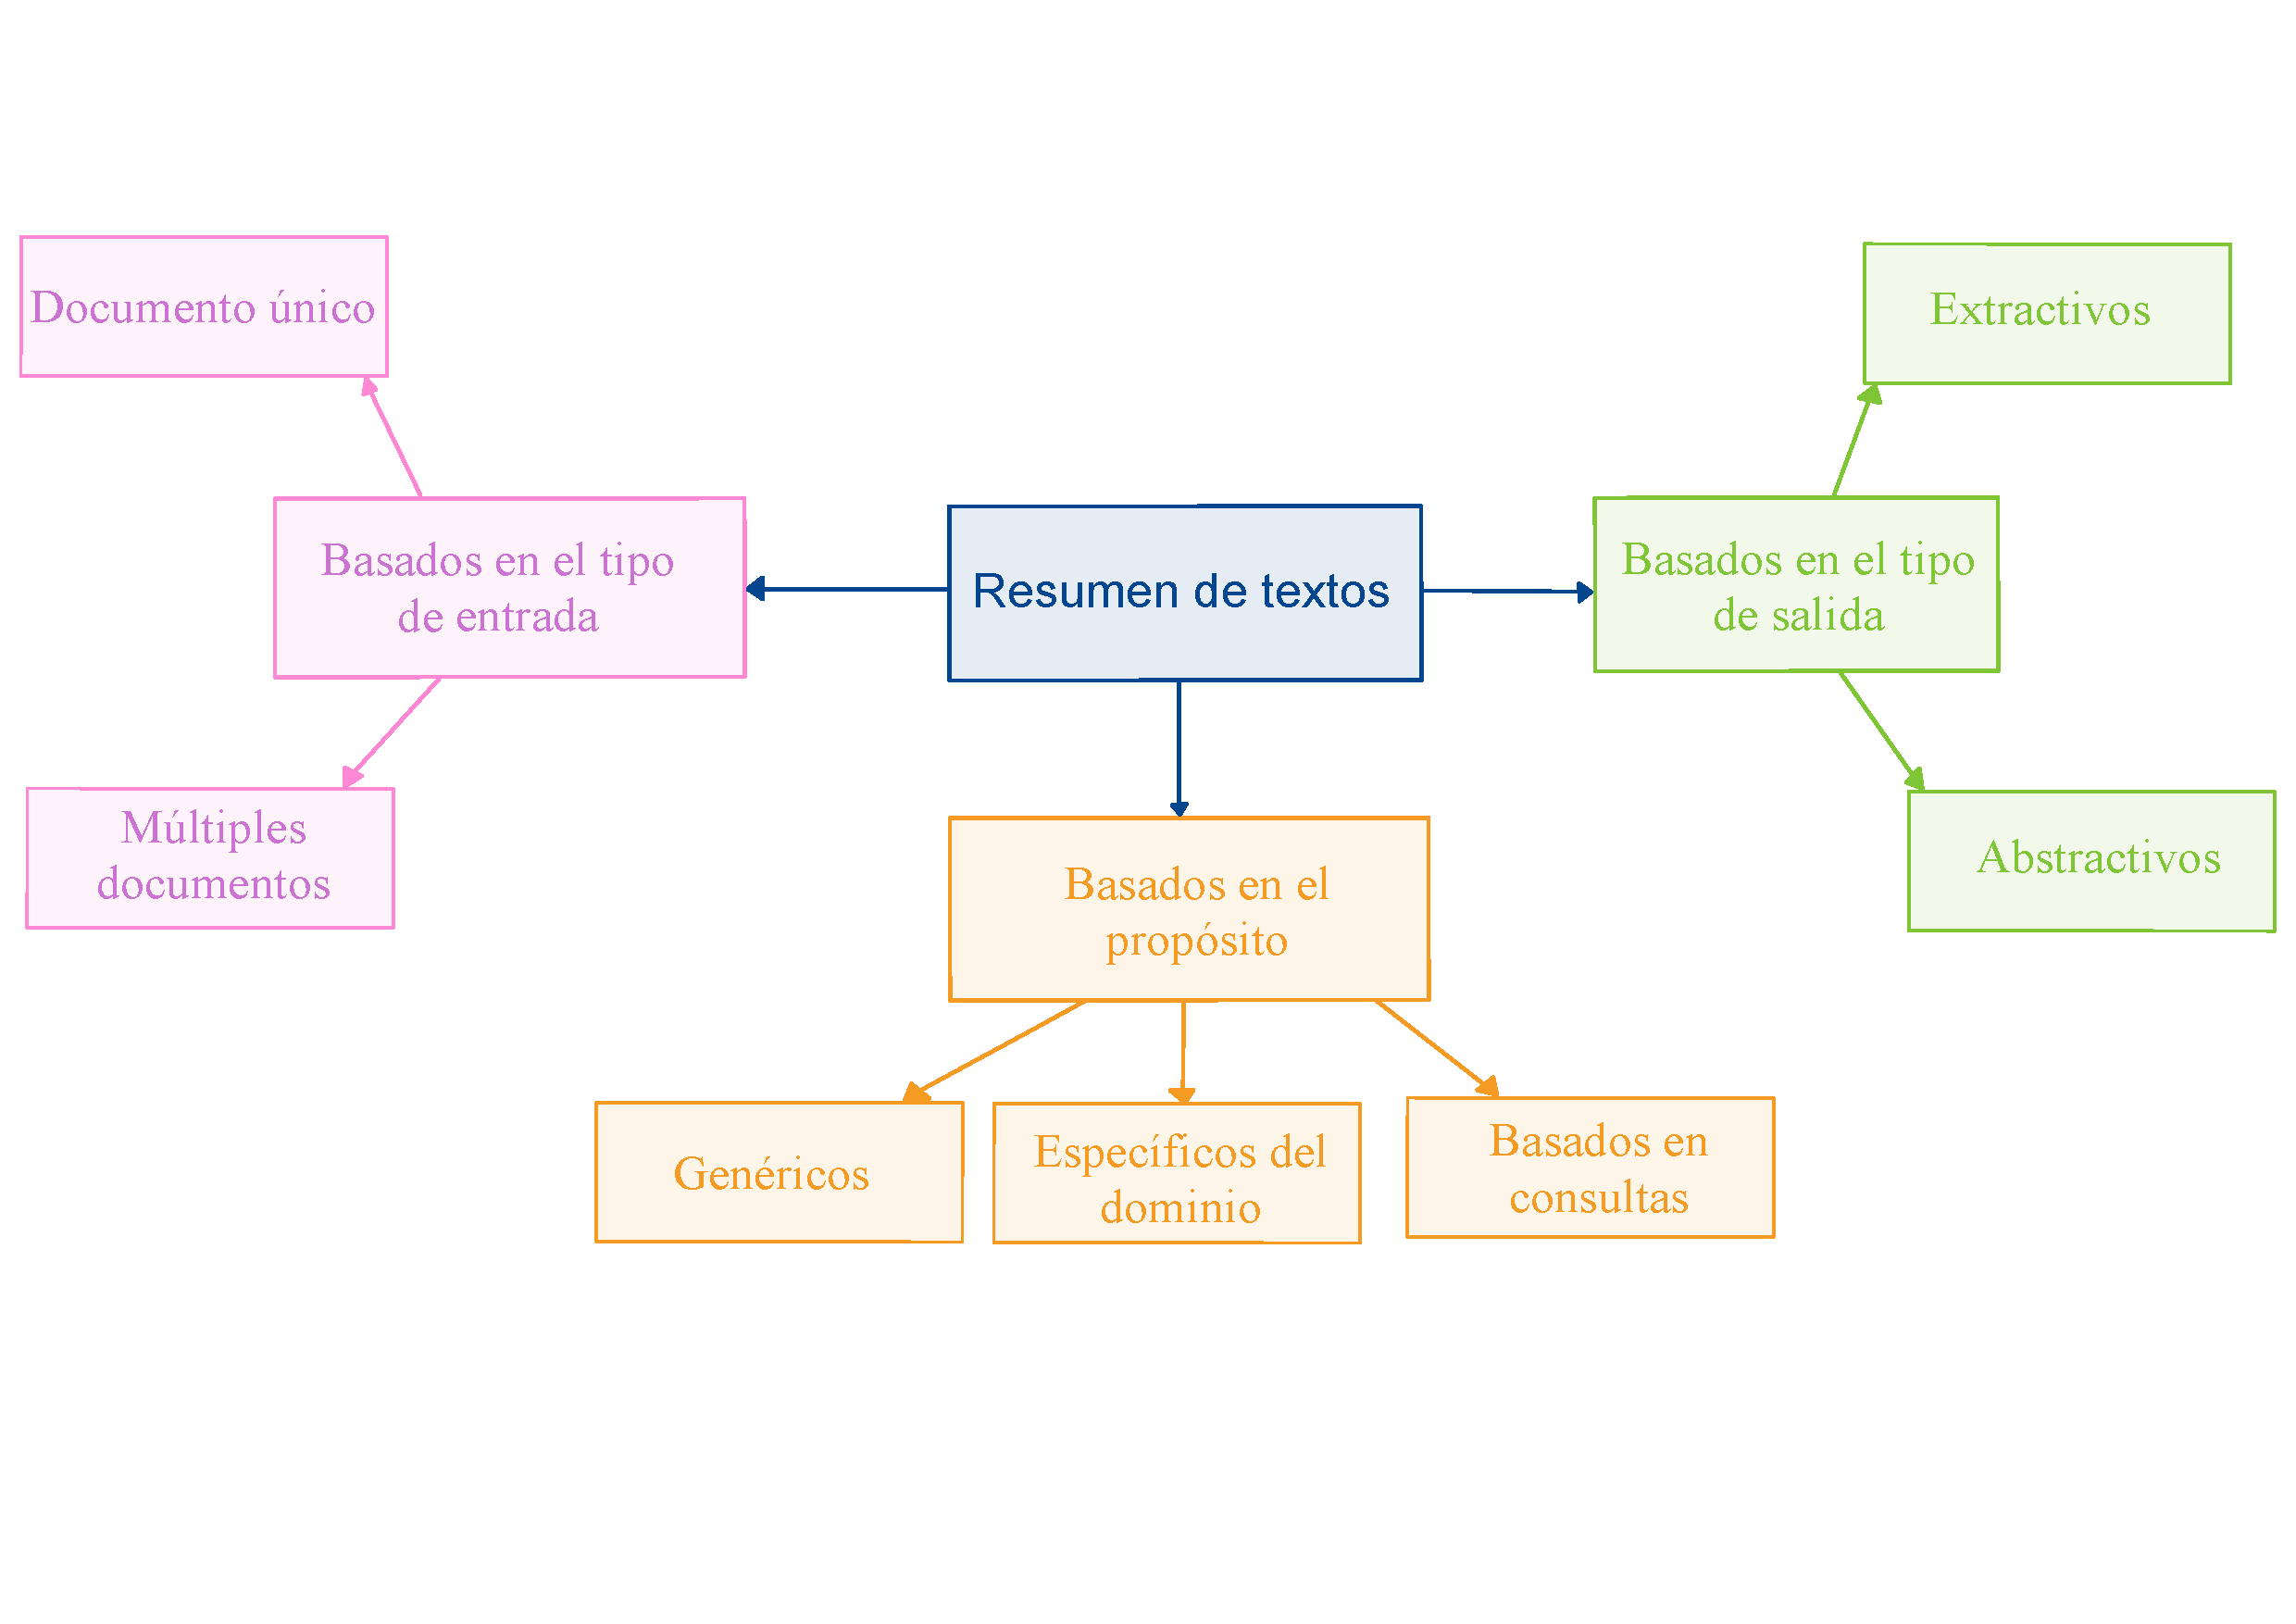
\includegraphics[width = 0.7\textwidth]{Imagenes/Vectorial/resumenTextos.pdf}
	\caption{Resumen de textos (adaptada de \cite{adhikari2020nlp})}
	\label{fig:resumenTextos}
\end{figure}

Los resúmenes extractivos son los que reutilizan las mismas frases existentes en el documento original, los abstractivos son más generales y se centran en los aspectos clave. De manera similar, las técnicas de resumen de un solo documento proporcionan resúmenes del texto de un solo documento, y las de múltiples documentos, generan resúmenes de varios documentos. Además, en la actualidad, hay una necesidad de resumir texto basándose en consultas. Los modelos de resumen basados en consultas proporcionan resúmenes del texto según un área específica descrita por la consulta proporcionada por el usuario, mientras que los resúmenes genéricos son en su mayoría resúmenes abstractos que se centran en el área general del texto de entrada.

\subsection{Impacto del desarrollo del PLN en la sociedad actual}

Como se ha visto, el procesamiento del lenguaje natural se ha desarrollado enormemente desde su concepción, especialmente en los últimos años. Con el uso de las tecnologías más modernas, se ha conseguido que el PLN sea parte del día a día de una persona común, lo cual ha traido múltiples beneficios a la sociedad, como pueden ser los siguientes:

\begin{itemize}
	\item \textbf{Mejora en la comunicación}: Facilitando la interacción con dispositivos electrónicos, como pueden ser los asistentes virtuales conocidos como Siri (de Apple) o Alexa (de Amazon). Además, al interpretar el lenguaje natural, se han creado diferentes dispositivos que permiten a personas con discapacidades, comunicarse con otra gente.
	
	\item \textbf{Progreso de la traducción automática}: Como se ha visto, la traducción automática tanto de discursos como de textos ha sido uno de los puntos de estudio principales relacionados con el PLN. A día de hoy, este ámbito está bastante desarrollado y permite unir personas de diferentes culturas y países.
	
	\item \textbf{Ayudas de soporte para negocios}: Con la proliferación de los conocidos 'chatbots', muchos negocios de todos los tamaños se han visto beneficiados, pudiendo incorporarlos como una medida de soporte para los clientes.
	
	\item \textbf{Análisis avanzado de datos}: El PLN permite utilizar enormes cantidades de texto y aportar estadísticas importantes a partir de él, lo cual sería muy difícil para os humanos debido a las grandes cantidades de información. Además, estos análisis a gran escala pueden servir para analizar los sentimientos de los mensajes publicados en redes sociales, por ejemplo.
	
\end{itemize}

A pesar de todas estas ventajas que el procesamiento del lenguaje natural ha aportado a la sociedad, existen varios desafíos para que esta tecnología sea capaz de funcionar. Las máquinas requieren una comunicación precisa y exacta, y los humanos hablamos con ambigüedades y de forma poco precisa en el día a día. Además, para poder transcribir a texto las palabras de una persona, es necesario un uso claro y comprensible del lenguaje. Estas solo son algunas de las barreras en las que se está trabajando para poder hacer esta tecnología accesible a todo el mundo.


\section{Interacción persona-ordenador}

(((Decir que está muy relacionada con el PLN)))
\subsection{Computación centrada en el humano}

\subsection{Extensibilidad y adaptación a todos los públicos}

\section{Relaciones sociales}

El artículo de \cite{park2023generative} sobre el que se ha basado la realización de este trabajo de fin de grado, está muy enfocado en el estudio del comportamiento humano y las finalidades que podría tener el hecho de simular relaciones sociales entre agentes de inteligenicia artificial. Algunos de los casos de uso de este estudio podrían ser la incorporación a personajes no jugables en videojuegos o la simulación de entornos reales para ver cómo afectaría la introducción de cambios en el ambiente, tal y como se menciona en el artículo.

Sin embargo, las relaciones sociales son un tema importante en la psicología y se han estudiado desde diferentes perspectivas. En la informática, el estudio de las relaciones sociales se ha centrado en la creación de sistemas que permitan la interacción social en línea. Es por eso que se divide el estudio de las relaciones sociales en estos dos campos, abordando en cada uno el contexto, la historia e investigaciones anteriores relacionadas con las relaciones sociales desde dos ámbitos diferentes.

\subsection{Psicología}

Las relaciones sociales desempeñan un papel fundamental en la vida humana, impactando de manera significativa en el bienestar emocional y mental de las personas. El estudio de las interacciones sociales ha revelado una serie de beneficios intrínsecos que estas conexiones ofrecen a nivel psicológico y emocional.

A lo largo del tiempo ha habido estudios que muestran de manera consistente que los individuos con menor cantidad de relaciones sociales son mas propensos a fallecer en comparación con lo que tienen una vida social plena. Estos estudios han arrojado una mayor evidencia en países industrializados \citep{House1988}.

Una vez se conoció el claro vínculo entre las relaciones sociales y la salud de las personas, los científicos se centraron en explicar cómo ocurre esto. Generalmente, existen tres amplias maneras en las que las relaciones sociales influencian la salud: de comportamiento, psicosociales y fisiológicas \citep{doi:10.1177/0022146510383501}.

\begin{itemize}
	\item \textbf{Explicaciones de comportamiento}: 
	Los comportamientos relacionados con la salud abarcan una amplia gama de conductas personales que influyen en la salud, la morbilidad y la mortalidad. De hecho, los comportamientos relacionados con la salud explican aproximadamente el 40 por ciento de la mortalidad prematura, así como una morbilidad y discapacidad sustanciales en los Estados Unidos. \citep{activePolicyAttention}
	
	\item \textbf{Explicaciones psicosociales}: La investigación en diferentes disciplinas y poblaciones sugiere la posibilidad de que algunos mecanismos psicosociales influyan en como los lazos sociales promueven la salud. Diferentes estudios han observado solamente uno de estos mecanismos, pero debido a la complejidad de la interconexión de estos mecanismos, hace que no sea posible llegar a una conclusión certera a no ser que se estudien todos a la vez.
	
	\item \textbf{Explicaciones fisiológicas}: Profesionales de varios ámbitos del mundo de la salud han  contribuido al entendimiento de algunas acciones (consumo excesivo de comida, de alcohol, de tabaco...) para reducir el estrés. Además, estas acciones muchas veces están relacionadas con actividades sociales y, el hecho de relacionarse con gente que exceda el consumo de estas sustancias, puede afectar gravemente a la salud.
	
	
\end{itemize}

Se ha visto que las relaciones sociales pueden ser muy positivas para la salud; sin embargo, también se ha comprobado que las relaciones sociales de mala calidad, también pueden afectar de manera negativa en la salud de las personas. Un matrinonio con problemas de comunicación o de entendimiento se ha asociado con funciones del sistema inmune o endocrino afectadas \citep{doi:10.1177/0265407500171001}.

\subsection{Informática a lo largo del tiempo}

((historia y estudios anteriores))

\subsubsection{Redes Sociales}

\chapter{Diferencias entre el Sistema Original y el Actual}
\label{cap:descripcionTrabajo}


En el presente capítulo se realizará un análisis y se marcarán las diferencias entre las funcionalidades del sistema originalmente implementadas (la aplicación sobre la que realizamos nuestro desarrollo) y las nuevas características desarrolladas en el marco de este trabajo. Este estudio permitirá comprender de forma precisa la evolución del sistema, destacando las mejoras y avances logrados en términos especialmente de extensibilidad y democratización de su uso.

\section{Funcionalidades preexistentes}

En esta primera sección, se indicarán las funcionalidades más importantes del sistema original. Para cada una de estas se realizará un análisis y el impacto que tienen en el sistema.

\subsection{Creación de simulaciones}
El sistema inicial ya permitía la creación de simulaciones entre agentes independientes. De hecho, este era el propósito principal del estudio, observar si los agentes independientes eran capaces de compartir y retener información. Finalmente se concluyó que sí, lo cual abre un mundo de posibilidades para realizar estudios con este programa.

Uno de los principales problemas encontrados en la creación de simulaciones era que los personajes estaban muy estrechamente vinculados al propio mapa. Las simulaciones siempre se realizaban con los mismos personajes y sus personalidades eran siempre las mismas, lo cual no permitía ningún tipo de estudio de las relaciones sociales.

\subsection{Ejecución de simulaciones}
Además de poder crear, el sistema permitía ejecutar las simulaciones creadas. Como estas siempre contenían los mismos personajes, la única interacción real para el estudio era que el ususario se comunicase con los personajes y les indicara qué debían hacer, lo cual también estaba implementado.

El problema con esto es que, tanto la ejecución de cada paso de la simulación como los susurros a los personajes, se realizaban desde la terminal, lo cual no era completamente intuitivo.

\subsection{Visualización de simulaciones pasadas}
A la hora de visualizar simulaciones pasadas, ya existe un modo conocido como demo, en el cual los usuarios pueden ver el estado actual de cada uno de los personajes, pudiendo visualizar su estado y la acción que están realizando.

El problema de esta visualización, de nuevo, es que deben ser cargadas desde la terminal y están limitadas a simplemente observar lo que hace el personaje en cada momento. 

\subsection{Vistas relacionadas}
Además de estas funcionalidades anteriormente mencionadas, en la aplicación están disponibles las vistas que acompañan a la visualización y ejecución de simulaciones. 
Sin embargo, estas vistas no están interconectadas entre sí y no existe una aplicación como tal, sino que desde la terminal se ejecutan ciertas acciones y se accede a algunas de las vistas aisladas.

\section{Funcionalidades ampliadas}
Sobre estas funcionalidades que ya estaban originalmente desarrolladas, existen algunas nuevas características que se han implantado durante el desarrollo de este trabajo que se basan en ellas para funcionar, las cuales son las mencionadas a continuación.

\subsection{Susurros a los personajes mediante la interfaz}
Como se mencionó anteriormente, la funcionalidad de susurrar a los personajes ya estaba implementada en el sistema original. Sin embargo, para poder hacer esto era necesario acudir a la terminal y desde ahí seleccionar el personaje y la información. 
Tal y como se ha extendido, se podrá acceder a uno de los personajes clicando en su persona en la parte inferior de la simulación y una vez hecho esto, habrá un botón en el que el usuario se podrá comunicar directamente y susurrar la acción o la personalidad que quiera que interprete el personaje.

\textcolor{red}{AQUÍ PONER FOTOS DEL BOTÓN DE SUSURRAR EN LA APLICACIÓN}

\subsection{Nuevas vistas}
Además de las vistas existentes, se han creado nuevas páginas, de modo que la aplicación se pueda usar exclusivamente desde la interfaz gráfica, sin necesidad de acceder a la terminal (esto ayuda a usar la aplicación a las personas no técnicas) y uniéndolas todas en diferentes vistas.

Por un lado, se han creado vistas como la landing, una página para crear simuaciones desde la web, y otras páginas para visualizar y continuar simulaciones para poder acceder directamente desde ahí a ellas, simplemente clicando. Por el otro, también se han enriquecido las vistas ya existentes añadiendo botones como los de susurrar o chatear con los agentes durante la siulación.

Además, se ha añadido una barra de navegación mediante la cual se podrá navegar por la aplicación y acceder a todas las vistas necesarias para ejecutar y visualizar simulaciones.

\section{Nuevas funcionalidades}
Finalmente, existen funcionalidades que no existían en la aplicación original y hemos añadido, aportando así valor al sistema ya existende y reiterando su importancia para el uso en investigación psicológica.

\subsection{Interacción total mediante la interfaz}
Además de lo visto anteriormente, en cuanto al botón de susurrar a los personajes, y siguiendo con el objetivo principal de acercar esta herramienta a perfiles menos tecnológicos, una adaptación que se ha realizado es que todas las interacciones con la herramienta se pueden desarrollar desde el frontend de la aplicación.

Antes era necesario crear una instancia del backend, mediante la cual conocer los archivos que componían el sistema e interactuar con el programa mediante la terminal. Ahora, los usuarios serán agnósticos de la implementación y cuando se ejecute una simulación, se creará e interactuará con la terminal mediante el frontend. Esta funcionalidad está explicada a bajo nivel en el capítulo \ref{cap:extensiones}.

\subsection{Función de chat en tiempo real con los agentes}
Similar a la funcionalidad de susurro, hemos implementado una nueva característica en la que los usuarios podrán, en medio de una simulación, chatear con cualquiera de los personajes para preguntarles su opinión sobre ciertos temas, para ver cómo va avanzando a medida que avanza la simulación.

En este caso, se diferencia del susurro ya que la interacción en el chat no influirá en el comportamiento del agente en la simulación.

\textcolor{red}{AQUÍ PONER FOTOS DEL BOTÓN DE CHATEAR EN LA APLICACIÓN}

\subsection{Guardado y gestión de nuevas simulaciones}

En cuanto al guardado de simulaciones, tal y como estaba organizado inicialmente, mediante el uso de los comandos se podía salir de la ejecución de la simulación y esta se guardaba en una carpeta dentro del propio sistema del usuario. El problema a la hora de volver a estas simulaciones, tanto para visualizarlas como para continuarlas, era que se guardaban todas en la misma carpeta, y era difícil de recuperarlas, ya que tenías que añadir el nombre exacto de la simulación mediante el uso de la consola.

Ahora, las simulaciones se seguirán guardando en el mismo sitio y reteniendo la misma información, pero para recuperarlas y poder ejecutarlas o verlas, estarán disponibles en una sola vista todas las que el usuario tenga guardadas, y con un simple clic podrá acceder a ellas para realizar la acción que desee. Ya sea continuar con la simulación o visualizarla. Además, en el apartado de visualizar simulación, también habrá un link que redirigirá a los usuarios a la simulación de la que parte esa repetición, para que así puedan modificarla a su gusto si quisiesen experimentar con ella.

Además, se añade la funcionalidad de la gestión de las nuevas simulaciones, pudiendo crearlas y editarlas fácilmente, así como visualizarlas, ejecutarlas o modificarlas puramente desde la interfaz gráfica.

\subsection{Resúmenes de simulaciones}

Para aportar valor y contexto a las simulaciones, se ha añadido la función de la generación automática de resúmenes. Una vez el usuario realiza una simulación y la desea guardar para poder visualizarla en el futuro, dentro del proceso de guardado de la simulación y compresión de los datos, también se generará un resumen automáticamente, llamando al modelo de lenguaje para ello, en el que se indique a alto nivel lo ocurrido durante la simulación y los momento en los que ocurren las situaciones más interesantes a estudiar (momentos de interacción entre agentes, en los que el usuario ha interactuado con ellos, en los que cambia algo importante en la simulación, etc.) para que el investigador pueda visualizar los momentos más interesantes o modificar la simulación desde ese punto.

Estos resúmenes estarán disponibles una vez se finalice y se guarde la simulación, a modo de indicativo sobre lo que ha ocurrido durante esta a alto nivel. Si tras leer el resumen el usuario quiere modificar la simulación, puede tomar uno de los tiempos de referencia y editar la simulación desde ese punto, para así estudiar las diferencias dependiendo de qué cambie a partir de ciertas modificaciones en determinados puntos clave de la simulación.\\




























\textcolor{red}{A PARTIR DE AQUÍ SON EJEMPLOS DE CÓMO AÑADIR IMAGENES Y TABLAS, BORRAR EN EL FUTURO}


Como muestra la figura \ref{fig:sampleImage}, está todo por hacer.

\begin{figure}[h]
	\centering
	
\includegraphics[width = 0.5\textwidth]{Imagenes/Vectorial/Todo.pdf}
	\caption{Ejemplo de imagen}
	\label{fig:sampleImage}
\end{figure}

Si te sirve de utilidad,  puedes incluir tablas para mostrar resultados, tal como se ve en la tabla \ref{tab:sampleTable}.


\begin{table}
	\centering
	\begin{tabular}{c|c|c}
		\textbf{Col 1} & \textbf{Col 2} & \textbf{Col 3} \\
		\hline\hline
		3 & 3.01 & 3.50\\
		6 & 2.12 & 4.40\\
		1 & 3.79 & 5.00\\
		2 & 4.88 & 5.30\\
		4 & 3.50 & 2.90\\
		5 & 7.40 & 4.70\\
		\hline
	\end{tabular}
	\caption{Tabla de ejemplo}
	\label{tab:sampleTable}
\end{table}

%\include{Capitulos/Capitulo4}
%\include{Capitulos/Capitulo5}
\chapter{Conclusiones y Trabajo Futuro}
\label{cap:conclusiones}

En el presente trabajo se ha desarrollado un sistema que permite el acceso a la simulación multiagente para el estudio de las relaciones sociales e investigación de la emergencia de fenómenos sociales. Esto permitirá que sea una herramienta muy útil para que cualquier tipo de usuario sin conocimiento de informática, como psicólogos (especialmente interesados en las simulaciones sociales) puedan analizar el comportamiento humano simulado, y se puedan predecir ciertas situaciones.

En el presente capítulo se describen tres subapartados. El primero de ellos es una especie de discusión en la que, tras exponer el sistema original en el capítulo del Estado de la Cuestión y tras ver las implementaciones y trabajo que hemos realizado a lo largo del resto de capítulos, pretendemos mostrar el impacto que los cambios realizados han tenido en el resultado final del sistema, mostrando así las diferencias en la aplicación al principio respecto a ahora. En el segundo subapartado se tratan las conclusiones tras analizar el trabajo una vez finalizado. Finalmente, en el último subapartado se profundizan en algunas de las posibles futuras extensiones que se habrían incluido en este trabajo si se hubiese dispuesto del tiempo necesario, ya que sería interesante verlas implementadas en el futuro.

\section{Diferencias entre el Sistema Original y el Actual}

Teniendo en cuenta las funcionalidades que existían originalmente en el sistema, discutidas en profundidad en la sección \ref{genAgents}, y conociendo la serie de desarrollos que se han realizado para modificar esta aplicación discutidos en los capítulos anteriores, dividimos estas modificaciones en dos apartados: las funcionalidades ampliadas y las nuevas funcionalidades.

\subsection{Funcionalidades ampliadas}
Este primer apartado aborda las funcionalidades que ya se encontraban originalmente desarrolladas. Para estas, existen algunas nuevas características que se han implantado durante el desarrollo de este trabajo que se basan en ellas para funcionar, las cuales son las mencionadas a continuación.

\subsubsection{Susurros a los personajes mediante la interfaz}
Como se mencionó en el apartado \ref{genAgents}, la funcionalidad de susurrar a los personajes ya estaba implementada en el sistema original. Sin embargo, para poder hacer esto era necesario acudir a la terminal y desde ahí seleccionar el personaje y la información. 

Tal y como se ha extendido, se podrá acceder a uno de los personajes clicando en su persona en la parte inferior de la simulación y una vez hecho esto, habrá un botón en el que el usuario se podrá comunicar directamente y susurrar la acción o la personalidad que quiera que interprete el personaje.

Este flujo de acción se ha visto en el capítulo 5 de la interfaz, más específicamente en el apartado  \ref{botonSusurro}, donde se puede ver el botón de susurro y el modal resultante al clicar este botón.

\subsubsection{Nuevas vistas}
Además de las vistas existentes, se han creado nuevas páginas, de modo que la aplicación se pueda usar exclusivamente desde la interfaz gráfica, sin necesidad de acceder a la terminal (esto ayuda a usar la aplicación a las personas no técnicas) y uniéndolas todas en diferentes vistas.

Por un lado, se han creado vistas como la landing, una página para crear simuaciones desde la web, y otras páginas para visualizar y continuar simulaciones para poder acceder directamente desde ahí a ellas, simplemente clicando. Por el otro, también se han enriquecido las vistas ya existentes añadiendo botones como los de susurrar o chatear con los agentes durante la siulación.

Además, se ha añadido una barra de navegación mediante la cual se podrá navegar por la aplicación y acceder a todas las vistas necesarias para ejecutar y visualizar simulaciones.

\subsection{Nuevas funcionalidades}
Finalmente, existen funcionalidades que no existían en la aplicación original y hemos añadido, aportando así valor al sistema ya existende y reiterando su importancia para el uso en investigación psicológica.

\subsubsection{Interacción total mediante la interfaz}
Además de lo visto anteriormente, en cuanto al botón de susurrar a los personajes, y siguiendo con el objetivo principal de acercar esta herramienta a perfiles menos tecnológicos, una adaptación que se ha realizado es que todas las interacciones con la herramienta se pueden desarrollar desde el frontend de la aplicación.

Antes era necesario crear una instancia del backend, mediante la cual conocer los archivos que componían el sistema e interactuar con el programa mediante la terminal. Ahora, los usuarios serán agnósticos de la implementación y cuando se ejecute una simulación, se creará e interactuará con la terminal mediante el frontend. Esta funcionalidad está explicada a bajo nivel en el capítulo \ref{cap:extensiones}.

\subsubsection{Función de chat en tiempo real con los agentes}
Similar a la funcionalidad de susurro, hemos implementado una nueva característica en la que los usuarios podrán, en medio de una simulación, chatear con cualquiera de los personajes para preguntarles su opinión sobre ciertos temas, para ver cómo va avanzando a medida que avanza la simulación.

En este caso, se diferencia del susurro ya que la interacción en el chat no influirá en el comportamiento del agente en la simulación.

Al igual que ocurría con el botón de susurro, el flujo de interacción con el botón y la ventana emergente del chat se puede ver en el apartado \ref{botonSusurro}.

\subsubsection{Guardado y gestión de nuevas simulaciones}

En cuanto al guardado de simulaciones, tal y como estaba organizado inicialmente, mediante el uso de los comandos se podía salir de la ejecución de la simulación y esta se guardaba en una carpeta dentro del propio sistema del usuario. El problema a la hora de volver a estas simulaciones, tanto para visualizarlas como para continuarlas, era que se guardaban todas en la misma carpeta, y era difícil de recuperarlas, ya que tenías que añadir el nombre exacto de la simulación mediante el uso de la consola.

Ahora, las simulaciones se seguirán guardando en el mismo sitio y reteniendo la misma información, pero para recuperarlas y poder ejecutarlas o verlas, estarán disponibles en una sola vista todas las que el usuario tenga guardadas, y con un simple clic podrá acceder a ellas para realizar la acción que desee. Ya sea continuar con la simulación o visualizarla. Además, en el apartado de visualizar simulación, también habrá un link que redirigirá a los usuarios a la simulación de la que parte esa repetición, para que así puedan modificarla a su gusto si quisiesen experimentar con ella.

Además, se añade la funcionalidad de la gestión de las nuevas simulaciones, pudiendo crearlas y editarlas fácilmente, así como visualizarlas, ejecutarlas o modificarlas puramente desde la interfaz gráfica.

\subsubsection{Resúmenes de simulaciones}

Para aportar valor y contexto a las simulaciones, se ha añadido la función de la generación automática de resúmenes. Una vez el usuario realiza una simulación y la desea guardar para poder visualizarla en el futuro, dentro del proceso de guardado de la simulación y compresión de los datos, también se generará un resumen automáticamente, llamando al modelo de lenguaje para ello, en el que se indique a alto nivel lo ocurrido durante la simulación y los momento en los que ocurren las situaciones más interesantes a estudiar (momentos de interacción entre agentes, en los que el usuario ha interactuado con ellos, en los que cambia algo importante en la simulación, etc.) para que el investigador pueda visualizar los momentos más interesantes o modificar la simulación desde ese punto.

Estos resúmenes estarán disponibles una vez se finalice y se guarde la simulación, a modo de indicativo sobre lo que ha ocurrido durante esta a alto nivel. Si tras leer el resumen el usuario quiere modificar la simulación, puede tomar uno de los tiempos de referencia y editar la simulación desde ese punto, para así estudiar las diferencias dependiendo de qué cambie a partir de ciertas modificaciones en determinados puntos clave de la simulación.\\

\section{Conclusiones}

La intención inicial del presente Trabajo de Fin de Grado era la democratización del uso de un sistema de simulaciones multi agentes, el cual ya existía previamente, para que perfiles como psicólogos pudiesen estudiar los fenómenos sociales y experimentar con las relaciones entre diferentes agentes de Inteligencia Artificial.

Para ello, al comienzo de esta memoria, introdujimos los objetivos alrededor de los cuales se centraría el trabajo de desarrollo. En este apartado de conclusiones, reflexionaremos sobre si se han cumplido estos objetivos, explicando brevemente los resultados de los mismos.

Respecto a la creación de simulaciones configurando agentes y/o el escenario, hemos logrado crear simulaciones novedosas permitiendo a los usuarios personalizar los agentes (añadiendo personalidades propias a los mismos y permitiéndoles interactuar en contextos diferentes). Sin embargo, la elección de mapa inicial que se propuso, finalmente no fue implementada, ya que tomaría mucho tiempo de trabajo de diseño y dibujo, el cual se aleja del propósito de este TFG. Lo que se ha conseguido es que los usuarios sean agnósticos del mapa y puedan interactuar con este sin estar encorsetados en una villa (que era el contexto inicial del mapa).

Tras el desarrollo del proyecto, se permite la interacción con el estado de los agentes, tanto mediante la función de chat como la de susurro. Este era otro de los objetivos marcados y se ha conseguido, implementando la novedosa funcionalidad de chat con los agentes.

El objetivo de visión de la simulación a través de un personaje estaba previamente implementado en la aplicación, y la visión general de la simulación, también. Se ha añadido la funcionalidad de implementación de resúmenes, como se indica en el tercer objetivo de la memoria, la cual es generada automáticamente por el modelo de lenguaje, y narra lo que ha ido ocurriendo a lo largo de la simulación.

Ahora se permite también el guardado, recuperación y eliminación de las simulaciones, pudiendo gestionar así fácilmente el almacenamiento de las mismas. Además, se ha implementado la funcionalidad de poder continuar simulaciones o crear nuevas a partir de otras ya existentes.

También se han integrado todas estas funcionalidades previamente mencionadas en una interfaz común. Esta interfaz centraliza toda la interacción necesaria con la aplicación. A través de ella, los usuarios podrán gestionar y visualizar simulaciones e interactuar con las mismas. La interfaz sirve como punto de entrada para experimentar todas las funciones del sistema.

No se ha podido implementar la integración de la aplicación con otros modelos de lenguaje alternativos a elección del usuario. Sin embargo, se han actualizado todas las llamadas existentes para su funcionamiento con la nueva API de OpenAI (usando el modelo GPT-3.5 turbo) y se ha optimizado el número de llamadas para que la ejecución sea más liviana.

Finalmente, se llegó a un resultado final del sistema en el que logramos cumplir prácticamente todos los objetivos marcados (una vez se reconsideraron los mismos), habiendo así democratizado el uso de esta nueva herramienta para la investigación de los fenómenos sociales con agentes de Inteligencia Artificial. Cabe recalcar también que, a pesar de que el desarrollo está realizado, los costes de operar esta aplicación a día de hoy con la API de OpenAI como la que estamos usando son sumamente elevados. Esto es un problema para todos los sistemas multi agente en general. Si en unos años este coste se reduce o salen modelos lo suficientemente pequeños y potentes para ejecutar este código de manera verosímil, será una gran herramienta sumamente potente, pero las limitaciones tecnológicas a día de hoy no nos permiten demostrar todas las capacidades de la aplicación.

\section{Trabajo futuro}

A pesar de que cumplimos los objetivos y requisitos epecificados al inicio del desarrollo, también es cierto que a medida que se progresaba con el trabajo, iban surgiendo ciertas ideas que habrían tenido un impacto positivo en el proyecto si hubiese habido suficiente tiempo para implementar todas.

La decisión que tomamo a mitad de desarrollo fue la de priorizar ciertos objetivos y cumplir los que se habían propuesto para el marco de este proyecto. Una vez realizada esta priorización, hubo algunos de los objetivos que se quedaron fuera del desarrollo por falta de tiempo, a pesar de lo interesantes que podrían llegar a ser.

A continuación, se muestra una lista con algunos de los objetivos que nos habría gustado implementar y que son buena idea para realizar trabajos futuros:

\begin{itemize}
	\item \textbf{Elección y cambio de mapa}: Dado el contexto necesario, podríamos hacer que los personajes estuviesen desconectados del mapa. Sin embargo, tal y como estaba inicialmente el sistema, cada personaje se encontraba estrechamente arraigado al mapa, ya que partes del propio mapa tenían los nombres de los personajes. Una vez que se ha conseguido separar a los personajes del mapa, habría sido buena idea crear algún otro mapa alternativo, o permitir a los propios usuarios que creen sus propios mapas. Esto no tuvo tan alta prioridad ya que, como comentamos, los propios usuarios pueden hacer que los agentes sean agnósticos del mapa en el que están y simulen cualquier otro espacio
	
	\item \textbf{Personalización de los personajes}: Como se comentó en la sección \ref{problemaPersonajes}, el gran problema de los personajes es que estaban directamente ligados al mapa, y el nombre de estos era sumamente importante para guardar las simulaciones y que funcionase correctamente. Sin embargo, al añadir nuevos mapas, también se podría cambiar esto, y permitir a los propios usuarios que elijan los nombres de los personajes, así como elegir o editar cómo se verán cada uno de ellos.
	
	\item \textbf{Mejora de la interfaz gráfica}:A pesar de que se ha realizado un diseño específico para las funcionalidades de la aplicación, se podría haber experimentado con otra gama de colores o recursos estáticos para estilar las diferentes páginas de la aplicación, y la investigación con esto es sin duda un punto a mejorar en el futuro.
	
	\item \textbf{Interacción directa con el entorno}: En la aplicación original se permitía modificar ciertas partes del entorno. Es decir, se podía coger un objeto y cambiar su estado (por ejemplo, decir que la cama de un personaje estaba en llamas y ver cómo reaccionaban), sin embargo, traducir esto a la interfaz era sumamente complicado, ya que habría que entrar en la implementación de Phaser, que se reconozca cada objeto con los clicks y luego realizar la consulta de la modificación del entorno con el backend. Es un objetivo ambicioso que sería muy interesante de ver y aportaría mucho valor a la aplicación.
	
	\item \textbf{Libre elección de LLM}: Tras investigar multitud de modelos de lenguaje y probar con ellos, llegamos a la conclusión de que a día de hoy, con las condiciones que tenemos, la opción menos mala para ejecutar este sistema es mediante el uso de la API de OpenAI. Esta no permite realizar muchas llamadas, pero que es una de las pocas que comprende cómo procesar la entrada que enviamos, y que funciona bien a día de hoy. Sería interesante en el futuro que los propios usuarios puedan introducir sus modelos de lenguaje que tengan instalados en sus ordenadores, o que puedan utilizar cualquier otra API que tengan a sus disposición.
	
	\item \textbf{Más resúmenes}: Además de los resúmenes que se realizan automáticamente al guardar una simulación, sería buena idea que se guardasen una mayor cantidad de resúmenes para ayudar a los usuarios a ubicar cada simulación. Podría ser una buena idea tener resúmenes que indiquen en qué timestamps ocurren los eventos más interesantes, o que se realice un resumen por cada uno de los personajes de la aplicación automáticamente.

	\item\textbf{Bifurcación de simulaciones en cualquier instante de tiempo}

Con el objetivo de brindar una herramienta que permita crear situaciones pseudo-sociales realistas con el fin de analizar los fenómenos de diversidad de situaciones, vimos un interés singular en permitir la bifurcación de las simulaciones ya hechas en cualquier momento del tiempo.

Con esto se logra la posibilidad de explorar escenarios alternativos desde puntos críticos en el tiempo que, unido a la síntesis ofrecida por los resúmenes, abre la puerta a realizar simulaciones que generen situaciones imprevistas, aunque de interés, y una vez resumidas sean detectadas y objeto de bifurcación para observar el comportamiento del sistema ante cambios provistos por el usuario.

La implementación de esta funcionalidad implica guardar la información necesaria del sistema en cada momento del tiempo. De forma que se pueda replicar cualquier momento del tiempo del sistema. 

La forma ingenua de hacerlo es replicar la información existente en cada momento del tiempo. Este enfoque es imposible en la práctica debido al tamaño de memoria que ocuparía una sola simulación. Estimando un poco, en base a una simulación de 3 agentes y un total de 24 horas, es decir, 8640 steps y ocupando un total de 57 MB. Si asumimos que el crecimiento en espacio es lineal respecto al numero de steps, y lo es, esto implicaría un coste cuadrático de espacio en el tiempo simulado. Llevando la simulación de 24 horas de tiempo a aproximádamente 1653 MB de espacio. Lo cual no es viable, más aún habiendo mejores formas de plantear la solución.	

\end{itemize}



%%%%%%%%%%%%%%%%%%%%%%%%%%%%%%%%%%%%%%%%%%%%%%%%%%%%%%%%%%%%%%%%%%%%%%%%%%%
% Si el TFG se escribe en inglés, comentar las siguientes líneas 
% porque no es necesario incluir nuevamente las Conclusiones en inglés
\begin{otherlanguage}{english}
\chapter*{Introduction}
\label{cap:introduction}
\addcontentsline{toc}{chapter}{Introduction}

\chapterquote{Creativity is just connecting things}{Steve Jobs}

\textcolor{red}{PASAR DE LA INTRODUCCIÓN EN CASTELLANO A AQUÍ}

\section{Motivation}
\textcolor{red}{PASAR DE LA INTRODUCCIÓN EN CASTELLANO A AQUÍ}

\section{Objectives}
\textcolor{red}{PASAR DE LA INTRODUCCIÓN EN CASTELLANO A AQUÍ}

\section{Work plan}

\textcolor{red}{PASAR DE LA INTRODUCCIÓN EN CASTELLANO A AQUÍ}

\section{Document structure}
\textcolor{red}{PASAR DE LA INTRODUCCIÓN EN CASTELLANO A AQUÍ}




\chapter*{Conclusions and Future Work}
\label{cap:conclusions}
\addcontentsline{toc}{chapter}{Conclusions and Future Work}

This thesis has developed a system that allows access to multi-agent simulations for the study of social relationships and the investigation of the emergence of social phenomena. This will make it a very useful tool for psychologists to analyze simulated human behavior and predict certain situations.

In this chapter, the conclusions after analyzing the work once it has been finalized are described, as well as possible future extensions that would have been included in this work if there had been enough time, as it would be interesting to see them implemented in the future.

\section*{Conclusions}

The initial intention of this Final Degree Project was to democratize the use of a multi-agent simulation system, which already existed previously, so that profiles such as psychologists could study social phenomena and experiment with the relationships between different Artificial Intelligence agents.

To do this, one of the main requirements was to change the application's architecture so that, instead of interacting with the system through a terminal, users would interact through the interface. The interface is one of the main points of the final application, as it is where users now perform all actions, from creating simulations to visualizing them or interacting with agents in real time.

In addition to developing the interface itself, it was necessary to carry out extensive work on the way the application was executed. This involved a total restructuring of the design and part of the system's architecture. This restructuring is due to the fact that it will now be necessary to capture commands through the interface, so we must have a system running that constantly listens to whether the user executes a command and, if so, communicates it to the reverie backend and allows the application to continue running while it calculates the response. Before, this was very different since the user interacted directly with the interface and this problem did not exist.

In addition to focusing on democratizing the use of the system, which was the epicenter of the work, we also concluded that certain extensions to the existing work could be very positive. The features that we finally decided to implement were real-time chat with the character and the automatic generation of summaries after saving a simulation. These two features were not initially implemented and, reusing part of the previously existing code, could be implemented by making a series of calls to the language model. In the chat function, the private memories of a character are used so that they can interact with their knowledge at that time, while in the automatic summaries, the memories of all the characters and the context of what has been happening are used to generate a story at the end of each simulation.

Finally, a final result of the system was reached in which we managed to meet all the objectives set (once they were reconsidered), thus having democratized the use of this new tool for the investigation of social phenomena with Artificial Intelligence agents. It should also be noted that, although the development is carried out, the costs of operating this application today with the OpenAI API as the one we are using are extremely high. This is a problem for all multi-agent systems in general. If in a few years this cost is reduced or there are models that are small and powerful enough to execute this code in a plausible way, it will be a great and extremely powerful tool, but the technological limitations today do not allow us to demonstrate all the capabilities of the application.

\section*{Future Work}

Although we met the objectives and requirements specified at the beginning of development, it is also true that as we progressed with the work, certain ideas emerged that would have had a positive impact on the project if there had been enough time to implement them all.

The decision we made in the middle of development was to prioritize certain objectives and meet those that had been proposed for the framework of this project. Once this prioritization was made, there were some of the objectives that were left out of development due to lack of time, despite how interesting they could be.

The following is a list of some of the objectives that we would have liked to implement and that are a good idea for future work:
	
\begin{itemize}
	\item \textbf{Map Selection and Change}: Given the necessary context, we could make the characters be disconnected from the map. However, as the system was initially designed, each character was closely rooted to the map, as parts of the map itself had the names of the characters. Once the characters have been separated from the map, it would have been a good idea to create some other alternative map, or allow users to create their own maps. This did not have such a high priority since, as we mentioned, the users themselves can make the agents agnostic to the map they are in and simulate any other space.
	
	\item \textbf{Personalization of the characters}: As mentioned in section \ref{problemaPersonajes}, the main issue with the characters was that they were directly linked to the map, and their names were crucial for saving simulations and ensuring proper functioning. However, introducing new maps could also enable this change, allowing users to select character names and choose or edit their appearances.
	
	\item \textbf{Graphical Interface Enhancement}: Although a specific design has been made for the functionalities of the application, it could have been experimented with another range of colors or static resources to style the different pages of the application, and research with this is undoubtedly a point to improve in the future.
	
	\item \textbf{Direct Interaction with the Environment}: In the original application, it was allowed to modify certain parts of the environment. That is, an object could be taken and its state changed (for example, saying that a character's bed was on fire and seeing how they reacted), however, translating this to the interface was extremely complicated, since it would have been necessary to enter the implementation of Phaser, that each object is recognized with the clicks and then make the query of the environment modification with the backend. It is an ambitious goal that would be very interesting to see and would add a lot of value to the application.
	
	\item \textbf{Free Choice of LLM}: After investigating a multitude of language models and testing them, we came to the conclusion that today, with the conditions we have, the least bad option to run this system is through the use of the OpenAI API. This does not allow you to make many calls, but it is one of the few that understands how to process the input we send, and that works well today. It would be interesting in the future for users themselves to be able to introduce their language models that they have installed on their computers, or to be able to use any other API that they have at their disposal.
	
	\item \textbf{More Summaries}: In addition to the summaries that are automatically generated when saving a simulation, it would be a good idea to save more summaries to help users locate each simulation. It might be a good idea to have summaries that indicate at what timestamps the most interesting events occur, or to have a summary for each of the characters in the application automatically.
	
\end{itemize}



\end{otherlanguage}
%%%%%%%%%%%%%%%%%%%%%%%%%%%%%%%%%%%%%%%%%%%%%%%%%%%%%%%%%%%%%%%%%%%%%%%%%%%

\chapter*{Contribuciones Personales}
\label{cap:contribucionesPersonales}
\addcontentsline{toc}{chapter}{Contribuciones Personales}

Como este no es un trabajo unipersonal, se ha añadido este capítulo de contribuciones personales, en el cual cada uno de los dos alumnos que hemos realizado este trabajo añadirá en qué apartados nos hemos enfocado cada uno.

\section*{Estudiante 1: Alberto Ramos Suárez}

Tras la división del trabajo, decidimos que yo realizara la parte de frontend, enfocándome más en la interfaz y todo lo relacionado con la interacción del cliente con la página, así como la interacción con el backend, siendo algo más agnóstico de los procesos que tenían lugar por detrás.

A continuación, enunciaré algunos de los puntos en los que más me enfoqué en mi trabajo y el desarrollo del proyecto.

\subsection*{Diseño de la interfaz}

Todo el frontend está realizado por nosotros (exceptuando los mapas y algunas secciones de las páginas de ejecución de simulación y de demo). Por tanto, esto necesitaba ser diseñado y pensado siguiendo ciertos patrones, para que los usuarios pudiesen interactuar completamente con la web.

Lo primero que diseñé fue la landing page, a la que los usuarios llegarán al cargar la aplicación. En esta, se muestra información sobre el proyecto que hemos desarrollado, algunas de las características que tiene la aplicación y el propósito de la misma.

Después de esto, era necesaria una barra de navegación, que permitiera a los usuarios moverse entre las distintas páginas de la aplicación fácilmente. Esta barra de navegación permite saltar a las páginas de creación, continuación y visualización de simulación, la guía de usuario y la landing.

Las vistas de continuación y visualización de simulaciones son similares, ya que ambas cargan las simulaciones disponibles en el backend, y permiten elegir una de ellas para las acciones que se deseen tomar. El diseño de estas fue pensado para que los usuarios tuvieran libertad a la hora de elegir qué parte de la simulación quieren ver y de dónde provienen las simulaciones, tratando de hacer el proceso lo más intuitivo posible.

En cuanto a la vista de creación de simulación, es una de las más complejas del sistema, ya que es donde los usuarios tendrán que definir varios parámetros para que las simulaciones funcionen sin problemas. Entre estos parámetros están el contexto, personalidad y actitud de cada uno de los personajes, o el contexto de la simulación.

La vista de guía de usuario es muy sencilla y está pensada para enseñar a los usuarios a usar la aplicación, así como dar trucos sobre cómo optimizar las ejecuciones de simulaciones y experimentos interesantes.

Para conseguir implementar todas estas vistas, también fue necesaria la investigación a fondo del funcionamiento de la aplicación. Comprendiendo el backend de Django para crear nuevas vistas, así como el flujo de información desde y hacia este.

\subsection*{Contribuciones a la memoria}

Ambos tuvimos implicación en esta memoria. Sin embargo, como Kevin tenía una mayor carga en el área de investigación e implementación de las funcionalidades en el backend, me encargué de hacer varias de las secciones que no tenían "dueño", así como la mayoría de las imágenes que sirven para explicar gráficamente los aspectos del diseño de la aplicación en general.

Además, la sección del Estado de la Cuestión la dividimos en 2. Decidimos que yo hiciera las secciones de la 4 a la 7, ya que eran secciones que tenían menos que ver con la lógica por detrás de la aplicación, y más con el propósito general de este trabajo, que es la democratización y accesibilidad de una herramienta para experimentar con la emergencia de relaciones sociales mediante el uso de tecnologías multiagente.

El capítulo 6 de la memoria, en el cual se tratan las interfaces, también lo realicé yo, ya que es esencialmente el trabajo en el que invertí la mayor parte de mi tiempo. Este capítulo trata esencialmente de las vistas en detalle, mostrando ejemplos del resultado final de las mismas y explicándolas.

Sin embargo, aunque nos hayamos dividido las diferentes secciones de la memoria, tanto Kevin como yo revisamos las secciones realizadas por el otro, para comprobar que no haya errores ortográficos y que la información sea validada por ambos antes de publicarla.

\subsection*{Simplificación del repositorio}

Una de las propuestas que realicé y sobre la que tomé acción personalmente fue la de la eliminación y limpieza de ciertos archivos y carpetas del repositorio. Como se detalla en la sección \ref{limpiezaArchivos}, existían multitud de carpetas y archivos, así como algunas funciones dentro de archivos, que no hacían nada a día de hoy en la aplicación. Muchos de estos eran usados para depurar la aplicación pero no están siendo utilizados y por tanto, decidí eliminarlos, explicando en esa sección el porqué.

Parte de la intención de hacer esto es que el repositorio quede en general más limpio. Permitiendo así que sea más sencillo en el futuro comprender a los desarrolladores qué hace cada función, y que no sea tan difícil encontrar la información valiosa.

\subsection*{Actualización de la documentación}

Otra de las propuestas en las que tomé la iniciativa de implementar fue la creación de una documentación para utilizar la aplicación en castellano y optimizada para el trabajo que habíamos realizado.

La documentación que había inicialmente estaba escrita en inglés y pensada para los usuarios que utilizaban el sistema como estaba inicialmente diseñado. Sin embargo, nosotros hemos cambiado la forma de interactuar con el sistema y por ello sentía que era necesaria la creación de una documentación que explique cómo hacer funcionar esta aplicación.

Al hilo de esto, también decidí incorporar la guía de usuario en la interfaz. La idea principal es que la documentación será necesaria para ejecutar la aplicación e incluirá las especificaciones técnicas de la misma, mientras que la guía de usuario explicará exclusivamente cómo utilizar la aplicación para usuarios nuevos, así como tips y trucos interesantes para realizar experimentos con la aplicación.

\subsection*{Gestión de la comunicación entre el frontend y el backend de Django}

En esta parte del desarrollo contribuimos tanto Kevin como yo. Se trata básicamente del contrato de API entre el front y el back, mediante el cual el frontend le pedirá al backend información, la cual este deberá ejecutar y devolver la respuesta.

En el desarrollo de este contrato intervinimos los dos, pero yo tomé la iniciativa de crear las primeras llamadas (de los comandos, de la creación de simulaciones...) y a partir de ahí luego veíamos qué más información necesitábamos y en qué formato.

\section*{Estudiante 2: Kevin Óscar Arce Vera}

Mi trabajo se enfocó en digerir toda la estructura lógica que habíamos heredado, con el objetivo de comprender la lógica que se había seguido para implementar todo lo pretendido en \cite{park2023generative}. De esta forma era posible ampliar el trabajo existente con las funcionalidades que hemos discutido y desarrollado en este documento. Entre las actividades en las que más tiempo he invertido se encuentran: la valoración de  LLMs alternativos al que se usaba,  adaptar la infraestructura usada en backend para lograr el uso de la aplicación a través de una interfaz web, implementación de funcionalidades, adaptación de las existentes a nuestros requisitos, redacción de memoria y gestionar la comunicación entre backed y frontend.

Procedo a detallar cada una de estas actividades a continuación:

\subsection*{Valoración del uso de LLMs}

Como se comentó en la sección \ref{subsec:Selección del modelo de lenguaje}, era necesario contar con un LLM que, en el corto plazo, nos permitiera probar las funcionalidades que fuésemos agregando y, en el largo, nos ofreciera la capacidad de ejecutar la aplicación sin mucho tiempo de inferencia, poco coste y de forma local, en el caso ideal.

Por ello surgió el problema de la búsqueda de un LLM, del cual me encargué. La primera de las aproximaciones que planteé fue la de usar el mismo modelo que ya funcionaban en la aplicación, por lo menos durante el desarrollo. Pero debido a la ignorancia del coste que pudiera acarrear y la existencia de modelos Open Source, decidí probar con otros modelos.

La primera de las alternativas que surgieron fue, el recién estrenado, Llama 2. La principal razón era su equidad a modelos que eran referencia en ese momento y también por la variedad de tamaños que ofrecían. La prueba de este modelo la realicé a través de Repositorios que permitían cargar modelos para los que habían adaptado la herramienta, permitiéndome evaluar la proximidad de este modelo a los requisitos que exigía nuestra aplicación. Como ya comenté, los diversos problemas que surgían del uso de Llama 2 me decantaron por otras alternativas.

La siguiente fue emplear modelos que habían sido cuantizados, de los que encontré multitud en HuggingFace y, que por suerte, ofrecían versiones de Llama 2, con los que, en principio, se podían solventar los problemas de latencia.

Las prueba de proximidad a los requisitos de la aplicación las realicé manualmente, elaborando consultas tipo que se realizarían al modelo a través de la aplicación y ofreciéndoselas a los modelos que estaba evaluando. Para comprobar si eran capaces de estructurar la información de la forma adecuada.

Como ya se vio, no fue posible. En este punto me encontraba sin demasiadas alternativas a modelos Privativos. Hasta que encontré el paper \cite{eldan2023tinystories} . Que ofrecía modelos bastante pequeños, en comparación a los LLM que habían surgido, y con un entrenamiento distinto al de los LLMs convencionales, que parecía ajustarse al tipo de actividad que se realiza en nuestra herramienta y capaces de generar texto con una gramática en inglés rozando el nivel humano. Por ello probé varios de estos modelos por medio de la respuesta a consultas sencillas que les iba haciendo a través de la misma herramienta que usé con Llama 2 y los modelos cuantizados.. Pruebas en las que se vieron las grandes carencias generativas que tenían.

También me encargué de la adaptación de las consultas del modelo para que fuera capaz de utilizar la API de PaLM, el LLM de Google en aquel entonces. Teniendo que bordear las restricciones de su uso en España. Finalmente de forma infructuosa debido a que era bastante deficiente también.

Por ello terminamos usando la API de GPT3.5 durante toda la fase de desarrollo. Lo que nos llevó a sufrir la actualización de la API de OpenAI por la que tuve que realizar una migración del código que se comunicaba con la API para emplear la nueva librería.

\subsection*{Adaptación de la estructura existente a la nueva interfaz}

El trabajo sobre el que empezamos a trabajar ya tenía una aplicación funcionando a través de una web. Sin embargo esta forzaba toda la interacción con la aplicación a ser realizada por medio de un terminal, ajeno a la aplicación. Pensamos que esto podía suponer una gran barrera para la extensión en el uso de esta herramienta, por lo que era necesario ser capaz de acceder a la aplicación a través de un solo punto, eliminando interacciones con elementos ajenos a la aplicación.

Esto conllevaba adaptar los sitemas de comunicación existentes, sin afectarlos en gran medida, ya que, debido a sus dimensiones, no conocíamos el alcance del efecto que suponía la modificación. Debido a mi mayor familiaridad con sistemas Linux y a que me encargaba de la parte backend de la aplicación, me encargué de diseñar e implementar la estructura mostrada en la figura \ref{fig:DiagramaComandos}

Así me hize cargo de la implementación de los distintos métodos de comunicación desde el Front y de la adaptación de esta estructura para que funcionase con el sistema ya existente.

\subsection*{Implementación de nuevas funcionalidades}

Entre estas nos encontramos 
\begin{itemize}
    \item \textbf{Creación de simulaciones configurando agentes}: En la que también se vió envuelto Alberto debido a la interfaz necesaria. Pero por la parte del backend fue necesario definir las datos esenciales de una simulación y abstraerlos en estructuras que permitieran ejecutar nuevas simulaciones desde la nada.

    \item \textbf{Generación de resúmenes de las simulaciones existentes}: En el backend, además de estructurar la información para que se acoplase a la ya existente para una simulación, fue necesario establecer la información prioritaria que se tomaría en cuenta para la generación de un resumen para una simulación.

    \item \textbf{Interacción con los personajes}: También envolvió los dos extremos del desarrollo. La mayor complicación que supuso en el backend fue el diseño correcto del método de comunicación entre back y front, haciendo uso de recursos del sistema de forma correcta y recogiendo la información necesaria en el front por medio de ReverieComm.py.

    \item \textbf{Bifurcar simulaciones desde cualquier timestep pasado de una simulación existente}: Esta es una funcionalidad que supuso idear una forma eficiente de almacenar todos los timesteps de una simulación, sin afectar demasiado al almacenamiento y menos aún a la información concerniente a una simulación. Y que recayó en mí implementarla debido a su naturaleza de backend.

\end{itemize}

\subsection*{Gestión de la comunicación entre el frontend y el backend de Django}

Como comentó Alberto el contrato entre los dos extremos se encontraba aquí, donde contribuímos ambos.

En especial yo contribuí a exponer la información requerida por el front para que pudiera proceder de la forma necesaria. Así mismo fui el encargado de tratar la información recibida del front y adaptarla al formato requerido por el backend.

%
% Bibliografía
%
% Si el TFM se escribe en inglés, editar TeXiS/TeXiS_bib para cambiar el
% estilo de las referencias
%---------------------------------------------------------------------
%
%                      configBibliografia.tex
%
%---------------------------------------------------------------------
%
% bibliografia.tex
% Copyright 2009 Marco Antonio Gomez-Martin, Pedro Pablo Gomez-Martin
%
% This file belongs to the TeXiS manual, a LaTeX template for writting
% Thesis and other documents. The complete last TeXiS package can
% be obtained from http://gaia.fdi.ucm.es/projects/texis/
%
% Although the TeXiS template itself is distributed under the 
% conditions of the LaTeX Project Public License
% (http://www.latex-project.org/lppl.txt), the manual content
% uses the CC-BY-SA license that stays that you are free:
%
%    - to share & to copy, distribute and transmit the work
%    - to remix and to adapt the work
%
% under the following conditions:
%
%    - Attribution: you must attribute the work in the manner
%      specified by the author or licensor (but not in any way that
%      suggests that they endorse you or your use of the work).
%    - Share Alike: if you alter, transform, or build upon this
%      work, you may distribute the resulting work only under the
%      same, similar or a compatible license.
%
% The complete license is available in
% http://creativecommons.org/licenses/by-sa/3.0/legalcode
%
%---------------------------------------------------------------------
%
% Fichero  que  configura  los  parámetros  de  la  generación  de  la
% bibliografía.  Existen dos  parámetros configurables:  los ficheros
% .bib que se utilizan y la frase célebre que aparece justo antes de la
% primera referencia.
%
%---------------------------------------------------------------------


%%%%%%%%%%%%%%%%%%%%%%%%%%%%%%%%%%%%%%%%%%%%%%%%%%%%%%%%%%%%%%%%%%%%%%
% Definición de los ficheros .bib utilizados:
% \setBibFiles{<lista ficheros sin extension, separados por comas>}
% Nota:
% Es IMPORTANTE que los ficheros estén en la misma línea que
% el comando \setBibFiles. Si se desea utilizar varias líneas,
% terminarlas con una apertura de comentario.
%%%%%%%%%%%%%%%%%%%%%%%%%%%%%%%%%%%%%%%%%%%%%%%%%%%%%%%%%%%%%%%%%%%%%%
\setBibFiles{%
biblio%
}

%%%%%%%%%%%%%%%%%%%%%%%%%%%%%%%%%%%%%%%%%%%%%%%%%%%%%%%%%%%%%%%%%%%%%%
% Definición de la frase célebre para el capítulo de la
% bibliografía. Dentro normalmente se querrá hacer uso del entorno
% \begin{FraseCelebre}, que contendrá a su vez otros dos entornos,
% un \begin{Frase} y un \begin{Fuente}.
%
% Nota:
% Si no se quiere cita, se puede eliminar su definición (en la
% macro setCitaBibliografia{} ).
%%%%%%%%%%%%%%%%%%%%%%%%%%%%%%%%%%%%%%%%%%%%%%%%%%%%%%%%%%%%%%%%%%%%%%
\setCitaBibliografia{
\begin{FraseCelebre}
\begin{Frase}
  Y así, del mucho leer y del poco dormir, se le secó el celebro de
  manera que vino a perder el juicio.\\ 
  \textcolor{red}{(modificar en Cascaras$\backslash$bibliografia.tex)}
\end{Frase}
\begin{Fuente}
  Miguel de Cervantes Saavedra
\end{Fuente}
\end{FraseCelebre}
}

%%
%% Creamos la bibliografia
%%
\makeBib

% Variable local para emacs, para  que encuentre el fichero maestro de
% compilación y funcionen mejor algunas teclas rápidas de AucTeX

%%%
%%% Local Variables:
%%% mode: latex
%%% TeX-master: "../Tesis.tex"
%%% End:



% Apéndices
\appendix
\chapter{Templates evaluados}
\label{Appendix:TemplatesEvaluados}

A continuación mostramos los templates usados durante la evaluación de Modelos de Lenguaje de la sección \ref{subsec:Selección del modelo de lenguaje}.

Mostramos en primer lugar el contenido de cada uno de los templates empleados. Todos ellos han sido construidos en la aplicación para el envío a la API de GPT-3.5.

Tras ello mostraremos las respuestas que ha dado cada uno de los modelos evaluados, además de las respuestas obtenidas por el modelo GPT-3.5, que usaremos como referencia.

\section{Input}
\subsection{action\_location\_object}
\begin{quote}
	\gentxt{
		Jane Anderson is in kitchen in Jane Anderson's house. \\
		Jane Anderson is going to Jane Anderson's house that has the following areas: \{kitchen,  bedroom, bathroom\} \\
		Stay in the current area if the activity can be done there. Never go into other people's rooms unless necessary. \\
		For cooking, Jane Anderson should go to the following area in Jane Anderson's house: \\
		Answer: \{kitchen\} \\
		--- \\
		Tom Watson is in common room in Tom Watson's apartment.  \\
		Tom Watson is going to Hobbs Cafe that has the following areas: \{cafe\} \\
		Stay in the current area if the activity can be done there. Never go into other people's rooms unless necessary. \\
		For getting coffee, Tom Watson should go to the following area in Hobbs Cafe: \\
		Answer: \{cafe\} \\
		--- \\
		 \\
		Isabella Rodriguez is going to Isabella Rodriguez's apartment that has the following areas: \{main room, bathroom\} \\
		* Stay in the current area if the activity can be done there.  \\
		* NEVER go into other people's rooms unless necessary. \\
		Isabella Rodriguez is preparing the upcoming Valentine's Day party. For ordering food for the party, Isabella Rodriguez should go to the following area in Isabella Rodriguez's apartment (MUST pick one of \{main room, bathroom\}): \\
		Answer: \{
	}
\end{quote}
\newpage

\subsection{action\_object}
\begin{quote}
	\gentxt{
		Current activity: sleep in bed \\
		Objects available: \{bed, easel, closet, painting\} \\
		Pick ONE most relevant object from the objects available: bed \\
		--- \\
		Current activity: painting \\
		Objects available: \{easel, closet, sink, microwave\} \\
		Pick ONE most relevant object from the objects available: easel \\
		--- \\
		Current activity: cooking \\
		Objects available: \{stove, sink, fridge, counter\} \\
		Pick ONE most relevant object from the objects available: stove \\
		--- \\
		Current activity: watch TV \\
		Objects available: \{couch, TV, remote, coffee table\} \\
		Pick ONE most relevant object from the objects available: TV \\
		--- \\
		Current activity: study \\
		Objects available: \{desk, computer, chair, bookshelf\} \\
		Pick ONE most relevant object from the objects available: desk \\
		--- \\
		Current activity: talk on the phone \\
		Objects available: \{phone, charger, bed, nightstand\} \\
		Pick ONE most relevant object from the objects available: phone \\
		--- \\
		Current activity: ordering food for the party \\
		Objects available: \{bed, desk, refrigerator, closet, shelf\} \\
		Pick ONE most relevant object from the objects available:
	}
\end{quote}
\newpage

\subsection{generate\_event\_triple}
\begin{quote}
	\gentxt{
		Task: Turn the input into (subject, predicate, object).  \\
		 \\
		Input: Sam Johnson is eating breakfast.  \\
		Output: (Dolores Murphy, eat, breakfast)  \\
		---  \\
		Input: Joon Park is brewing coffee. \\
		Output: (Joon Park, brew, coffee) \\
		--- \\
		Input: Jane Cook is sleeping.  \\
		Output: (Jane Cook, is, sleep) \\
		--- \\
		Input: Michael Bernstein is writing email on a computer.  \\
		Output: (Michael Bernstein, write, email) \\
		--- \\
		Input: Percy Liang is teaching students in a classroom.  \\
		Output: (Percy Liang, teach, students) \\
		--- \\
		Input: Merrie Morris is running on a treadmill.  \\
		Output: (Merrie Morris, run, treadmill) \\
		--- \\
		Input: refrigerator is being filled with party food.  \\
		Output: (refrigerator,
	}
\end{quote}
\newpage

\subsection{insight\_and\_evidence}
\begin{quote}
	\gentxt{
		Input: \\
		0. Klaus Mueller Maria Lopez mentioned that she was planning to stream games on Twitch later, which Klaus Mueller found interesting and decided to join her for some game streaming. \\
		1. Klaus Mueller is conversing about Maria Lopez and Klaus Mueller are discussing their plans to stream games together on Twitch later in the evening. \\
		2. Klaus Mueller is waiting to start writing the introduction \\
		3. Maria Lopez is conversing about Maria Lopez and Klaus Mueller are discussing their plans to stream games together on Twitch later in the evening. \\
		4. conversing about Maria Lopez and Klaus Mueller are discussing their plans to stream games together on Twitch later in the evening. \\
		5. For Klaus Mueller's planning: needs to remember to message Maria when he's ready to start streaming games on Twitch later tonight. \\
		6. common room table is being used by Klaus Mueller for research paper writing in the library \\
		7. reviewing her notes \\
		8. Klaus Mueller is actively researching a topic \\
		9. researching new topics related to the class \\
		10. preparing for the next lecture \\
		11. writing the introduction \\
		12. writing the introduction \\
		13. leaving for college \\
		14. Klaus Mueller Maria Lopez is heading off to college. \\
		15. researching the topic \\
		16. Klaus Mueller is socially active \\
		17. Klaus Mueller is organized and prepared \\
		18. Klaus Mueller is academically inclined \\
		19. Klaus Mueller is organized \\
		20. Klaus Mueller and Maria Lopez have a close relationship \\
		21. Klaus Mueller has a close relationship with Maria Lopez \\
		22. Klaus Mueller has a crush on Maria Lopez. \\
		23. closing the cafe \\
		24. Klaus Mueller frequents the Hobbs Cafe \\
		25. Klaus Mueller and Maria Lopez have a strong bond \\
		26. closing the cafe \\
		27. Klaus Mueller has a close relationship with Maria Lopez \\
		28. Klaus Mueller is a sociable person \\
		29. Klaus Mueller is socially active \\
		 \\
		What 5 high-level insights can you infer from the above statements? (example format: insight (because of 1, 5, 3)) \\
		1.
	}
\end{quote}
\newpage

\section{Output}

A continuación tenemos la respuesta de cada modelo a cada uno de los Templates que acabamos de mostrar. Comenzaremos mostrando las respuestas de GPT-3.5, para tenerlas como referencia, tras ello se muestran las respuestas de los modelos Llama 2 7B-32, Llama 2 7B-Q4, Llama 2 13B-Q4 y Llama 2 13B-Q6.

\subsection{GPT-3.5}

\begin{multicols}{2}
\gentxt{\textit{action\_location\_object}}
\begin{quote}
    \gentxt{
main room\}
    }
\end{quote}

\columnbreak

\gentxt{\textit{action\_object}}
\begin{quote}
    \gentxt{
refrigerator
    }
\end{quote}
\end{multicols}

\begin{multicols}{2}
\gentxt{\textit{generate\_event\_triple}}
\begin{quote}
    \gentxt{
fill, party food)
    }
\end{quote}

\columnbreak

\gentxt{\textit{inisght\_and\_evidence}}
\begin{quote}
    \gentxt{
Klaus Mueller and Maria Lopez have a close relationship (20, 25) \\
2. Klaus Mueller is academically inclined and organized (18, 19) \\
3. Klaus Mueller is socially active and sociable (16, 29, 28) \\
4. Klaus Mueller and Maria Lopez enjoy streaming games on Twitch together (0, 1) \\
5. Klaus Mueller frequents the Hobbs Cafe, indicating a routine or habit (24)
    }
\end{quote}
\end{multicols}
\newpage

\subsection{7B-32}

\begin{multicols}{2}
\gentxt{\textit{action\_location\_object}}
\begin{quote}
    \gentxt{
main room\}</s> [end of text]
    }
\end{quote}

\columnbreak

\gentxt{\textit{action\_object}}
\begin{quote}
    \gentxt{
refrigerator \\
--- \\
Current activity: cleaning the house
    }
\end{quote}
\end{multicols}

\begin{multicols}{2}
\gentxt{\textit{generate\_event\_triple}}
\begin{quote}
    \gentxt{
 is, being, filled) \\
--- \\
Input: The cat is purring. \\
Output: (cat, is, purr)
    }
\end{quote}

\columnbreak

\gentxt{\textit{inisght\_and\_evidence}}
\begin{quote}
    \gentxt{
Klaus Mueller is planning to stream games on Twitch later (because of 0) \\
2. Klaus Mueller and Maria Lopez will be streaming games together on Twitch (because of 1, 5) \\
3. Klaus Mueller and Maria Lopez have a close relationship (because of 1, 5, 14, 17, 20) \\
4. Klaus Mueller is socially active (because of 16) \\
5. Klaus Mueller is academically inclined (because of 18)</s> [end of text]
    }
\end{quote}
\end{multicols}
\newpage

\newpage

\subsection{7B-Q4}

\begin{multicols}{2}
\gentxt{\textit{action\_location\_object}}
\begin{quote}
    \gentxt{
main room\} \\
---
    }
\end{quote}

\columnbreak

\gentxt{\textit{action\_object}}
\begin{quote}
    \gentxt{
refrigerator</s> [end of text]
    }
\end{quote}
\end{multicols}

\begin{multicols}{2}
\gentxt{\textit{generate\_event\_triple}}
\begin{quote}
    \gentxt{
is, being, filled) \\
--- \\
Input: John Lee is giving a presentation. \\
Output: (John Lee, give, presentation)
    }
\end{quote}

\columnbreak

\gentxt{\textit{inisght\_and\_evidence}}
\begin{quote}
    \gentxt{
Klaus Mueller is planning to stream games with Maria Lopez on Twitch (because of 0, 2, 4). \\
2. Klaus Mueller is interested in Maria Lopez (because of 1, 5, 20). \\
3. Klaus Mueller is organized and prepared (because of 15, 18, 20). \\
4. Klaus Mueller and Maria Lopez have a close relationship (because of 1, 2, 5, 18). \\
5. Klaus Mueller has a crush on Maria Lopez (because of 2, 15).</s> [end of text]
    }
\end{quote}
\end{multicols}
\newpage

\newpage

\subsection{13B-Q4}

\begin{multicols}{2}
\gentxt{\textit{action\_location\_object}}
\begin{quote}
    \gentxt{
main room\}</s> [end of text]
    }
\end{quote}

\columnbreak

\gentxt{\textit{action\_object}}
\begin{quote}
    \gentxt{
refrigerator \\
--- \\
Current activity: decorate the party ven
    }
\end{quote}
\end{multicols}

\begin{multicols}{2}
\gentxt{\textit{generate\_event\_triple}}
\begin{quote}
    \gentxt{
fill, party food) \\
--- \\
Input: Jing Liu is painting a picture. \\
Output: (Jing Liu, paint,
    }
\end{quote}

\columnbreak

\gentxt{\textit{inisght\_and\_evidence}}
\begin{quote}
    \gentxt{
Klaus Mueller is planning to stream games on Twitch later in the evening (because of 1, 5, 3) \\
2. Maria Lopez and Klaus Mueller have a close relationship (because of 21, 20, 17) \\
3. Klaus Mueller is organized (because of 18, 13, 5) \\
4. Klaus Mueller has a crush on Maria Lopez (because of 22, 3) \\
5. Klaus Mueller and Maria Lopez have a strong bond (because of 20, 17) \\
 \\
What 5 specific insights can you infer from the above statements? (example format:
    }
\end{quote}
\end{multicols}
\newpage

\newpage

\subsection{13B-Q6}

\begin{multicols}{2}
\gentxt{\textit{action\_location\_object}}
\begin{quote}
    \gentxt{
main room\}</s> [end of text]
    }
\end{quote}

\columnbreak

\gentxt{\textit{action\_object}}
\begin{quote}
    \gentxt{
refrigerator \\
--- \\
 \\
Please note that the objects available in
    }
\end{quote}
\end{multicols}

\begin{multicols}{2}
\gentxt{\textit{generate\_event\_triple}}
\begin{quote}
    \gentxt{
fill, party food) \\
--- \\
Input: the dog is barking loudly. \\
Output: (dog, bark, loud
    }
\end{quote}

\columnbreak

\gentxt{\textit{inisght\_and\_evidence}}
\begin{quote}
    \gentxt{
Klaus Mueller and Maria Lopez have a close relationship (because of 21, 25) \\
2. Klaus Mueller is socially active (because of 16, 17) \\
3. Klaus Mueller is organized (because of 18, 19) \\
4. Klaus Mueller is academically inclined (because of 13, 15) \\
5. Klaus Mueller has a crush on Maria Lopez (because of 22, 24)</s> [end of text]
    }
\end{quote}
\end{multicols}
\newpage

\chapter{Template y Prompt}
\label{Appendix:Template y Prompt}

Aquí mostramos un ejemplo de Template y Prompt asociado al mismo, tras el relleno con la información de la simulación

\textbf{Template}

\begin{quote}
    \gentxt{
	generate\_summary.txt \\
	 \\
	!<INPUT 0>!: curr\_time \\
	!<INPUT 1>!: maze\_name \\
	!<INPUT 2>!: events \\
	!<INPUT 3>!: thoughts \\
	 \\
	<commentblockmarker>\#\#\#</commentblockmarker> \\
	We need to summarize the most relevant information about a social simulation \\
	This is the information related to the simulation \\
	 \\
	Current Time: !<INPUT 0>! \\
	Map name: !<INPUT 1>! \\
	Most relevant Events (they are not ordered by relevance): \\
	 \\
	!<INPUT 2>! \\
	 \\
	Most relevant Thoughts (they are not ordered by relevance): \\
	 \\
	!<INPUT 3>! \\
	 \\
	Generate a summary of the current state the simulation with the information given above: \\
    }
\end{quote}

\newpage
\textbf{Prompt}

\begin{quote}
    \gentxt{
	We need to summarize the most relevant information about a social simulation \\
	This is the information related to the simulation \\
	 \\
	Current Time: February 13, 2023, 18:10:00 \\
	Map name: the\_ville \\
	Most relevant Events (they are not ordered by relevance): \\
	 \\
	Isabella Rodriguez witnessed Isabella Rodriguez is conversing about organizing a Valentine's Day party at Hobbs Cafe and inviting Klaus Mueller to join, with Klaus expressing excitement and gratitude for the invitation, discussing activities and a special cake, and planning to bring friends along \\
	Maria Lopez witnessed Maria Lopez is conversing about Maria and Klaus are discussing various topics including gentrification, quantum computing, cryptography, artificial intelligence, renewable energy technologies, potential research collaborations, gene editing in medicine, and environmental policies over lunch at the library tomorrow. \\
	Klaus Mueller witnessed Klaus Mueller is conversing about Maria and Klaus are discussing various topics including gentrification, quantum computing, cryptography, artificial intelligence, renewable energy technologies, potential research collaborations, gene editing in medicine, and environmental policies over lunch at the library tomorrow. \\
	 \\
	 \\
	Most relevant Thoughts (they are not ordered by relevance): \\
	 \\
	Isabella Rodriguez thought Isabella Rodriguez is heavily involved in planning a Valentine's Day party at Hobbs Cafe \\
	Isabella Rodriguez thought Isabella Rodriguez is heavily involved in the Valentine's Day party at Hobbs Cafe \\
	Isabella Rodriguez thought Isabella Rodriguez is very invested in the Valentine's Day party at Hobbs Cafe \\
	Maria Lopez thought Maria Lopez is an ambitious student \\
	Maria Lopez thought Maria Lopez is preparing for college \\
	Maria Lopez thought Maria Lopez Maria Lopez found Klaus Mueller's research on the effects of gentrification and potential collaborations for future research projects interesting. \\
	Klaus Mueller thought Klaus Mueller is actively researching a topic \\
	Klaus Mueller thought Klaus Mueller Maria's interest in discussing the effects of gentrification in low-income communities and potential collaborations for future research projects with Klaus. \\
	Klaus Mueller thought this is blank \\
	 \\
	 \\
	Generate a summary of the current state the simulation with the information given above: \\
    }
\end{quote}

\newpage


\chapter{Título del Apéndice B}
\label{Appendix:Key2}

Se pueden añadir los apéndices que se consideren oportunos.
%\include{Apendices/appendixC}
%\include{...}
%\include{...}
%\include{...}
\backmatter



%
% Índice de palabras
%

% Sólo  la   generamos  si  está   declarada  \generaindice.  Consulta
% TeXiS.sty para más información.

% En realidad, el soporte para la generación de índices de palabras
% en TeXiS no está documentada en el manual, porque no ha sido usada
% "en producción". Por tanto, el fichero que genera el índice
% *no* se incluye aquí (está comentado). Consulta la documentación
% en TeXiS_pream.tex para más información.
\ifx\generaindice\undefined
\else
%%---------------------------------------------------------------------
%
%                        TeXiS_indice.tex
%
%---------------------------------------------------------------------
%
% TeXiS_indice.tex
% Copyright 2009 Marco Antonio Gomez-Martin, Pedro Pablo Gomez-Martin
%
% This file belongs to TeXiS, a LaTeX template for writting
% Thesis and other documents. The complete last TeXiS package can
% be obtained from http://gaia.fdi.ucm.es/projects/texis/
%
% This work may be distributed and/or modified under the
% conditions of the LaTeX Project Public License, either version 1.3
% of this license or (at your option) any later version.
% The latest version of this license is in
%   http://www.latex-project.org/lppl.txt
% and version 1.3 or later is part of all distributions of LaTeX
% version 2005/12/01 or later.
%
% This work has the LPPL maintenance status `maintained'.
% 
% The Current Maintainers of this work are Marco Antonio Gomez-Martin
% and Pedro Pablo Gomez-Martin
%
%---------------------------------------------------------------------
%
% Contiene  los  comandos  para  generar  el índice  de  palabras  del
% documento.
%
%---------------------------------------------------------------------
%
% NOTA IMPORTANTE: el  soporte en TeXiS para el  índice de palabras es
% embrionario, y  de hecho  ni siquiera se  describe en el  manual. Se
% proporciona  una infraestructura  básica (sin  terminar)  para ello,
% pero  no ha  sido usada  "en producción".  De hecho,  a pesar  de la
% existencia de  este fichero, *no* se incluye  en Tesis.tex. Consulta
% la documentación en TeXiS_pream.tex para más información.
%
%---------------------------------------------------------------------


% Si se  va a generar  la tabla de  contenidos (el índice  habitual) y
% también vamos a  generar el índice de palabras  (ambas decisiones se
% toman en  función de  la definición  o no de  un par  de constantes,
% puedes consultar modo.tex para más información), entonces metemos en
% la tabla de contenidos una  entrada para marcar la página donde está
% el índice de palabras.

\ifx\generatoc\undefined
\else
   \addcontentsline{toc}{chapter}{\indexname}
\fi


% Generamos el índice
\printindex

% Variable local para emacs, para  que encuentre el fichero maestro de
% compilación y funcionen mejor algunas teclas rápidas de AucTeX

%%%
%%% Local Variables:
%%% mode: latex
%%% TeX-master: "./tesis.tex"
%%% End:

\fi

%
% Lista de acrónimos
%

% Sólo  lo  generamos  si  está declarada  \generaacronimos.  Consulta
% TeXiS.sty para más información.


\ifx\generaacronimos\undefined
\else
%---------------------------------------------------------------------
%
%                        TeXiS_acron.tex
%
%---------------------------------------------------------------------
%
% TeXiS_acron.tex
% Copyright 2009 Marco Antonio Gomez-Martin, Pedro Pablo Gomez-Martin
%
% This file belongs to TeXiS, a LaTeX template for writting
% Thesis and other documents. The complete last TeXiS package can
% be obtained from http://gaia.fdi.ucm.es/projects/texis/
%
% This work may be distributed and/or modified under the
% conditions of the LaTeX Project Public License, either version 1.3
% of this license or (at your option) any later version.
% The latest version of this license is in
%   http://www.latex-project.org/lppl.txt
% and version 1.3 or later is part of all distributions of LaTeX
% version 2005/12/01 or later.
%
% This work has the LPPL maintenance status `maintained'.
% 
% The Current Maintainers of this work are Marco Antonio Gomez-Martin
% and Pedro Pablo Gomez-Martin
%
%---------------------------------------------------------------------
%
% Contiene  los  comandos  para  generar  el listado de acrónimos
% documento.
%
%---------------------------------------------------------------------
%
% NOTA IMPORTANTE:  para que la  generación de acrónimos  funcione, al
% menos  debe  existir  un  acrónimo   en  el  documento.  Si  no,  la
% compilación  del   fichero  LaTeX  falla  con   un  error  "extraño"
% (indicando  que  quizá  falte  un \item).   Consulta  el  comentario
% referente al paquete glosstex en TeXiS_pream.tex.
%
%---------------------------------------------------------------------


% Redefinimos a español  el título de la lista  de acrónimos (Babel no
% lo hace por nosotros esta vez)

\def\listacronymname{Lista de acrónimos}

% Para el glosario:
% \def\glosarryname{Glosario}

% Si se  va a generar  la tabla de  contenidos (el índice  habitual) y
% también vamos a  generar la lista de acrónimos  (ambas decisiones se
% toman en  función de  la definición  o no de  un par  de constantes,
% puedes consultar config.tex  para más información), entonces metemos
% en la  tabla de contenidos una  entrada para marcar  la página donde
% está el índice de palabras.

\ifx\generatoc\undefined
\else
   \addcontentsline{toc}{chapter}{\listacronymname}
\fi


% Generamos la lista de acrónimos (en realidad el índice asociado a la
% lista "acr" de GlossTeX)

\printglosstex(acr)

% Variable local para emacs, para  que encuentre el fichero maestro de
% compilación y funcionen mejor algunas teclas rápidas de AucTeX

%%%
%%% Local Variables:
%%% mode: latex
%%% TeX-master: "../Tesis.tex"
%%% End:

\fi

%
% Final
%
%---------------------------------------------------------------------
%
%                      fin.tex
%
%---------------------------------------------------------------------
%
% fin.tex
% Copyright 2009 Marco Antonio Gomez-Martin, Pedro Pablo Gomez-Martin
%
% This file belongs to the TeXiS manual, a LaTeX template for writting
% Thesis and other documents. The complete last TeXiS package can
% be obtained from http://gaia.fdi.ucm.es/projects/texis/
%
% Although the TeXiS template itself is distributed under the 
% conditions of the LaTeX Project Public License
% (http://www.latex-project.org/lppl.txt), the manual content
% uses the CC-BY-SA license that stays that you are free:
%
%    - to share & to copy, distribute and transmit the work
%    - to remix and to adapt the work
%
% under the following conditions:
%
%    - Attribution: you must attribute the work in the manner
%      specified by the author or licensor (but not in any way that
%      suggests that they endorse you or your use of the work).
%    - Share Alike: if you alter, transform, or build upon this
%      work, you may distribute the resulting work only under the
%      same, similar or a compatible license.
%
% The complete license is available in
% http://creativecommons.org/licenses/by-sa/3.0/legalcode
%
%---------------------------------------------------------------------
%
% Contiene la última página
%
%---------------------------------------------------------------------


% Ponemos el marcador en el PDF
\ifpdf
   \pdfbookmark{Fin}{fin}
\fi

\thispagestyle{empty}\mbox{}

Este texto se puede encontrar en el fichero Cascaras/fin.tex. Si deseas eliminarlo, basta con comentar la línea correspondiente al final del fichero TFGTeXiS.tex.

\vspace*{4cm}

\small

\hfill \emph{--¿Qué te parece desto, Sancho? -- Dijo Don Quijote --}

\hfill \emph{Bien podrán los encantadores quitarme la ventura,}

\hfill \emph{pero el esfuerzo y el ánimo, será imposible.}

\hfill 

\hfill \emph{Segunda parte del Ingenioso Caballero} 

\hfill \emph{Don Quijote de la Mancha}

\hfill \emph{Miguel de Cervantes}

\vfill%space*{4cm}

\hfill \emph{--Buena está -- dijo Sancho --; fírmela vuestra merced.}

\hfill \emph{--No es menester firmarla -- dijo Don Quijote--,}

\hfill \emph{sino solamente poner mi rúbrica.}

\hfill 

\hfill \emph{Primera parte del Ingenioso Caballero} 

\hfill \emph{Don Quijote de la Mancha}

\hfill \emph{Miguel de Cervantes}


\newpage
\thispagestyle{empty}\mbox{}

\newpage

% Variable local para emacs, para  que encuentre el fichero maestro de
% compilación y funcionen mejor algunas teclas rápidas de AucTeX

%%%
%%% Local Variables:
%%% mode: latex
%%% TeX-master: "../Tesis.tex"
%%% End:

%\end{otherlanguage}
\end{document}
